% Options for packages loaded elsewhere
\PassOptionsToPackage{unicode}{hyperref}
\PassOptionsToPackage{hyphens}{url}
%
\documentclass[
]{article}
\usepackage{lmodern}
\usepackage{amssymb,amsmath}
\usepackage{ifxetex,ifluatex}
\ifnum 0\ifxetex 1\fi\ifluatex 1\fi=0 % if pdftex
  \usepackage[T1]{fontenc}
  \usepackage[utf8]{inputenc}
  \usepackage{textcomp} % provide euro and other symbols
\else % if luatex or xetex
  \usepackage{unicode-math}
  \defaultfontfeatures{Scale=MatchLowercase}
  \defaultfontfeatures[\rmfamily]{Ligatures=TeX,Scale=1}
\fi
% Use upquote if available, for straight quotes in verbatim environments
\IfFileExists{upquote.sty}{\usepackage{upquote}}{}
\IfFileExists{microtype.sty}{% use microtype if available
  \usepackage[]{microtype}
  \UseMicrotypeSet[protrusion]{basicmath} % disable protrusion for tt fonts
}{}
\makeatletter
\@ifundefined{KOMAClassName}{% if non-KOMA class
  \IfFileExists{parskip.sty}{%
    \usepackage{parskip}
  }{% else
    \setlength{\parindent}{0pt}
    \setlength{\parskip}{6pt plus 2pt minus 1pt}}
}{% if KOMA class
  \KOMAoptions{parskip=half}}
\makeatother
\usepackage{xcolor}
\IfFileExists{xurl.sty}{\usepackage{xurl}}{} % add URL line breaks if available
\IfFileExists{bookmark.sty}{\usepackage{bookmark}}{\usepackage{hyperref}}
\hypersetup{
  pdftitle={Historical and Projected Water Balance Report for Little Saddle Mtn},
  pdfauthor={Janelle Christensen, Mike Tercek, David Thoma, John Gross},
  hidelinks,
  pdfcreator={LaTeX via pandoc}}
\urlstyle{same} % disable monospaced font for URLs
\usepackage[margin=1in]{geometry}
\usepackage{graphicx,grffile}
\makeatletter
\def\maxwidth{\ifdim\Gin@nat@width>\linewidth\linewidth\else\Gin@nat@width\fi}
\def\maxheight{\ifdim\Gin@nat@height>\textheight\textheight\else\Gin@nat@height\fi}
\makeatother
% Scale images if necessary, so that they will not overflow the page
% margins by default, and it is still possible to overwrite the defaults
% using explicit options in \includegraphics[width, height, ...]{}
\setkeys{Gin}{width=\maxwidth,height=\maxheight,keepaspectratio}
% Set default figure placement to htbp
\makeatletter
\def\fps@figure{htbp}
\makeatother
\setlength{\emergencystretch}{3em} % prevent overfull lines
\providecommand{\tightlist}{%
  \setlength{\itemsep}{0pt}\setlength{\parskip}{0pt}}
\setcounter{secnumdepth}{-\maxdimen} % remove section numbering

\title{Historical and Projected Water Balance Report for Little Saddle Mtn}
\author{Janelle Christensen, Mike Tercek, David Thoma, John Gross}
\date{8/3/2020}

\begin{document}
\maketitle

This data is based off of inmcm4 RCP 4.5 and HadGEM2-CC365 RCP 8.5 to
display projections for two potential climate futures. The historical
data uses gridmet. All data is sourced from a National Park Service data
set created by Mike Tercek, David Thoma and John Gross to predict
climate futures out to 2100 and report historical daymet and gridmet
data back to 1980 at the project level. A link to his original data set
can be found
\href{http://www.yellowstone.solutions/thredds/catalog.html}{here}.

\hypertarget{annual-values-through-time}{%
\subsection{Annual values through
time}\label{annual-values-through-time}}

These graphs, are shown in more detail later in this report. The
variables of runoff, rain, potential evapotranspiration (PET), actual
evapotranspiration (AET), and deficit are summed in the graphs that show
annual values through time. Accumulated snow water equivalent (SWE) and
accumulated growing degree days (AGDD) show the max value in the year,
and soil water shows the mean of the values.

The reason for the different mathematical evaluations is due to how
hydrologist look at these variables. Hydrologists accumulate water
variables that don't have an upper limit like rain runoff, and
evapostranspiration, whereas they average values that have an upper
limit like soil moisture. With soil moisture there is a limit to the
amount of water soil can hold based on soil water holding capacity that
is related to soil texture, rock fragments (that don't store water) and
soil depth. Temperature variables are averaged by convention and growing
degree days are summed to account for the seasonal accumulation of heat
that controls biological metabolism and thus growth rates and phenology
when water is available. For the variables that are accumulated, we take
the max of the varible because it is already a summation of the total
through the year.

\textbackslash begin\{figure\}

\{\centering \includegraphics{water_balance_graphs_files/figure-latex/unnamed-chunk-16-1}

\}

\textbackslash caption\{Figure 1. Annual averages over time. The gray
line represents historical data modeled from gridmet climate data, the
turquoise line represents and the yellow line represents
paste(model\_bc)\}\label{fig:unnamed-chunk-16}
\textbackslash end\{figure\}

\hypertarget{deficit-v.-actual-evapotranspiration-aet}{%
\subsection{Deficit v. Actual Evapotranspiration
(AET)}\label{deficit-v.-actual-evapotranspiration-aet}}

Deficit and Actual Evapotranspiration (AET) are the two best predictors
of vegetation type, and are useful variables in understanding what an
area may look like in the future. To understand why these variables are
such good predictors of vegetation, deficit can be understood as unmet
water need by plants and AET as the water used by vegetation. According
to Nathan Stevenson, AET and deficit are climatic controls of vegetation
distribution. If the clustering of AET and deficit change in climate
space, vegetation assemblages will respond and change to assemblages
adapted to the new climate space (1998). The figure below shows how AET
v. deficit changes for different habitat types.

\begin{figure}

{\centering 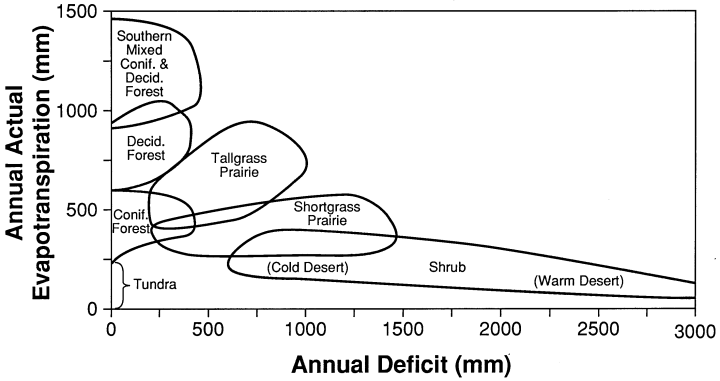
\includegraphics[width=0.5\linewidth]{aet_v_d} 

}

\caption{Stephenson (1998)}\label{fig:unnamed-chunk-17}
\end{figure}

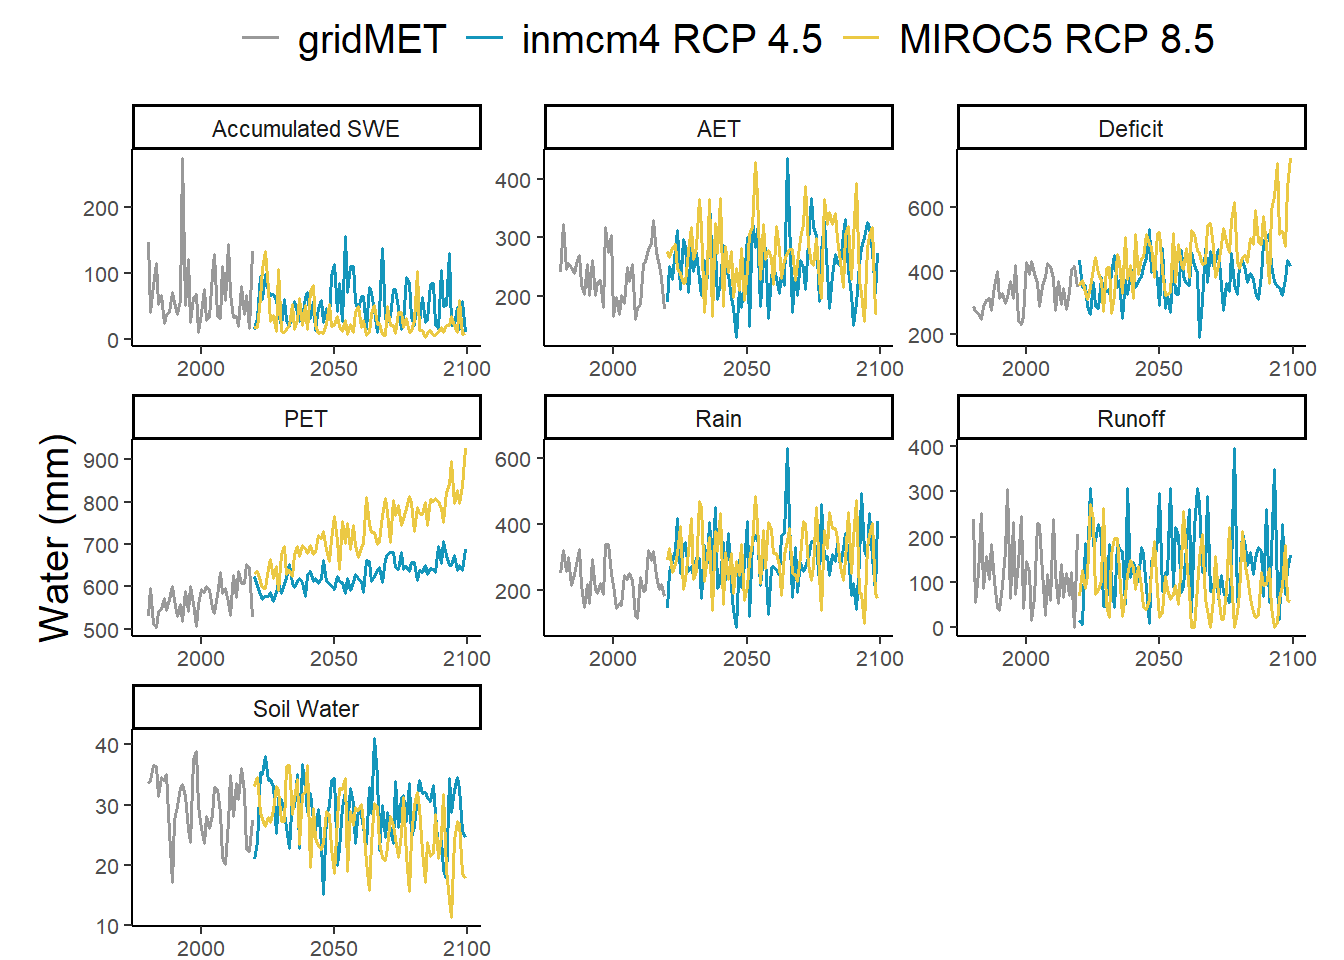
\includegraphics[width=0.5\linewidth]{water_balance_graphs_files/figure-latex/unnamed-chunk-18-1}
\includegraphics[width=0.5\linewidth]{water_balance_graphs_files/figure-latex/unnamed-chunk-18-2}

\hypertarget{soil-water}{%
\subsection{Soil Water}\label{soil-water}}

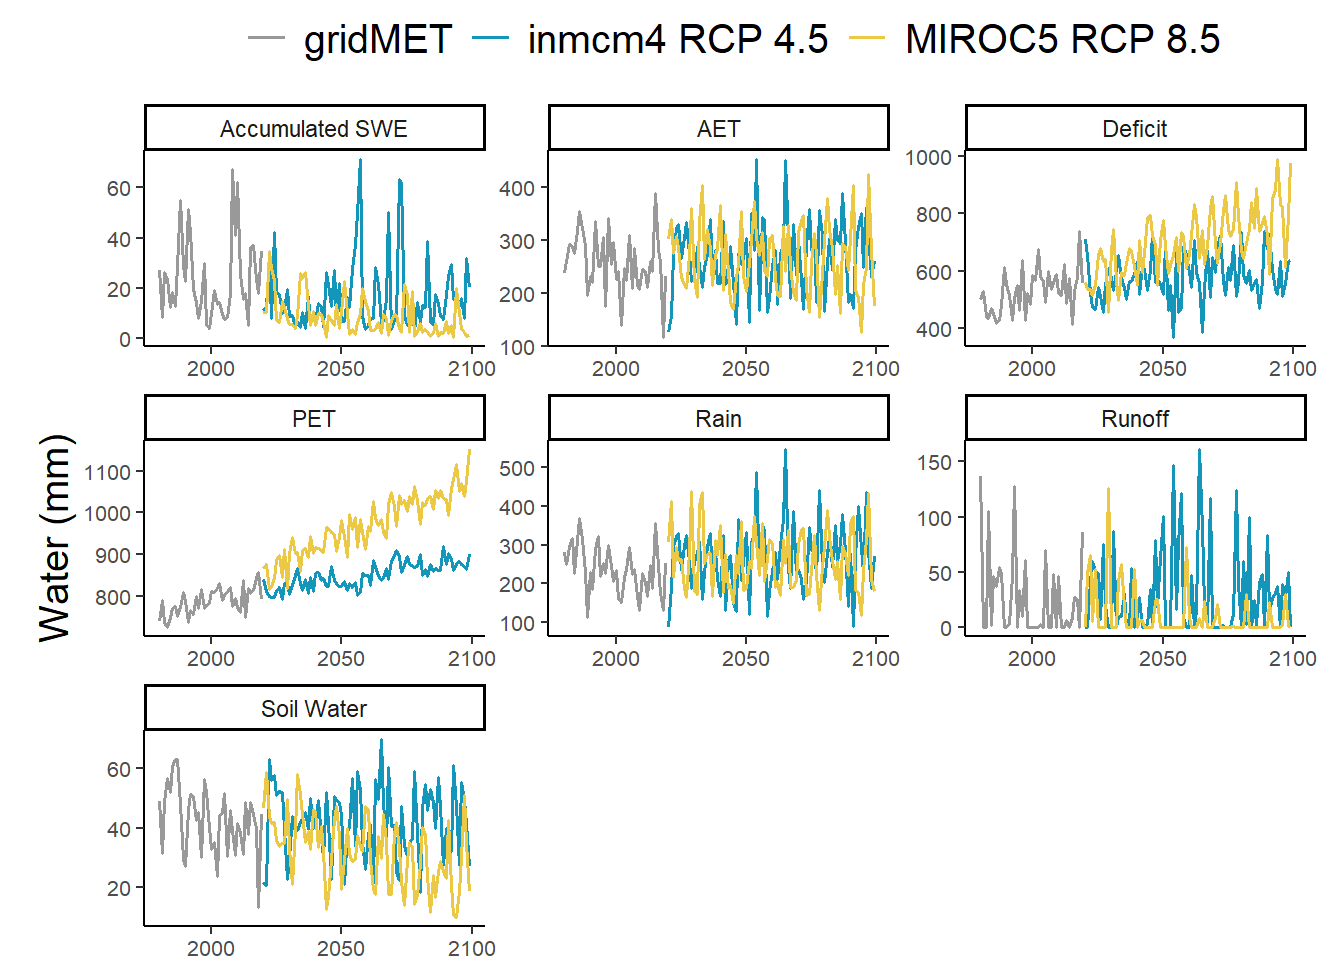
\includegraphics[width=0.5\linewidth]{water_balance_graphs_files/figure-latex/unnamed-chunk-19-1}
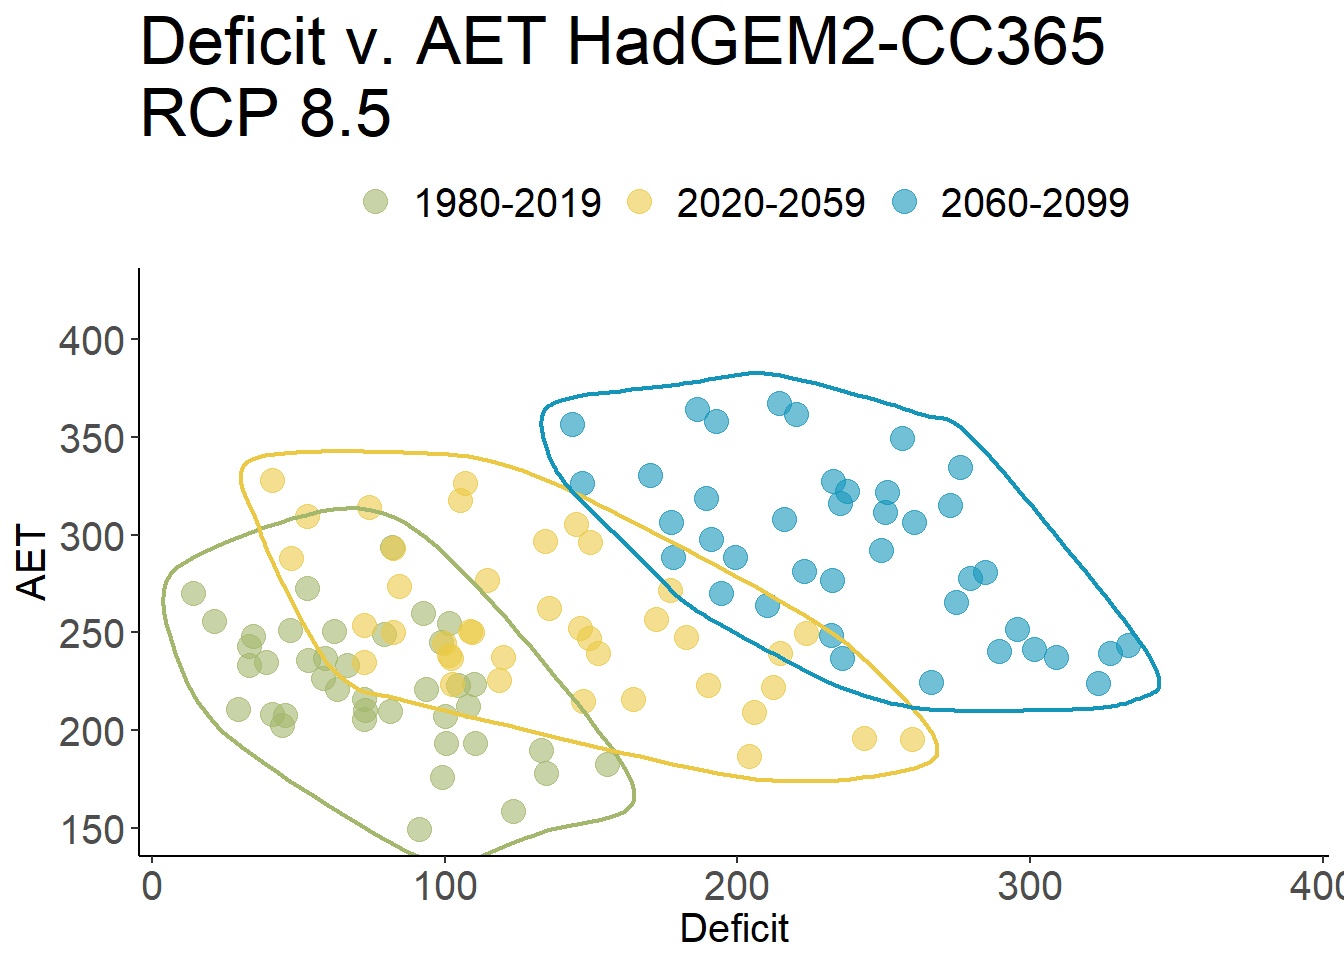
\includegraphics[width=0.5\linewidth]{water_balance_graphs_files/figure-latex/unnamed-chunk-19-2}
\includegraphics[width=0.5\linewidth]{water_balance_graphs_files/figure-latex/unnamed-chunk-19-3}
\includegraphics[width=0.5\linewidth]{water_balance_graphs_files/figure-latex/unnamed-chunk-19-4}
\includegraphics[width=0.5\linewidth]{water_balance_graphs_files/figure-latex/unnamed-chunk-19-5}
\includegraphics[width=0.5\linewidth]{water_balance_graphs_files/figure-latex/unnamed-chunk-19-6}

\hypertarget{runoff}{%
\subsection{Runoff}\label{runoff}}

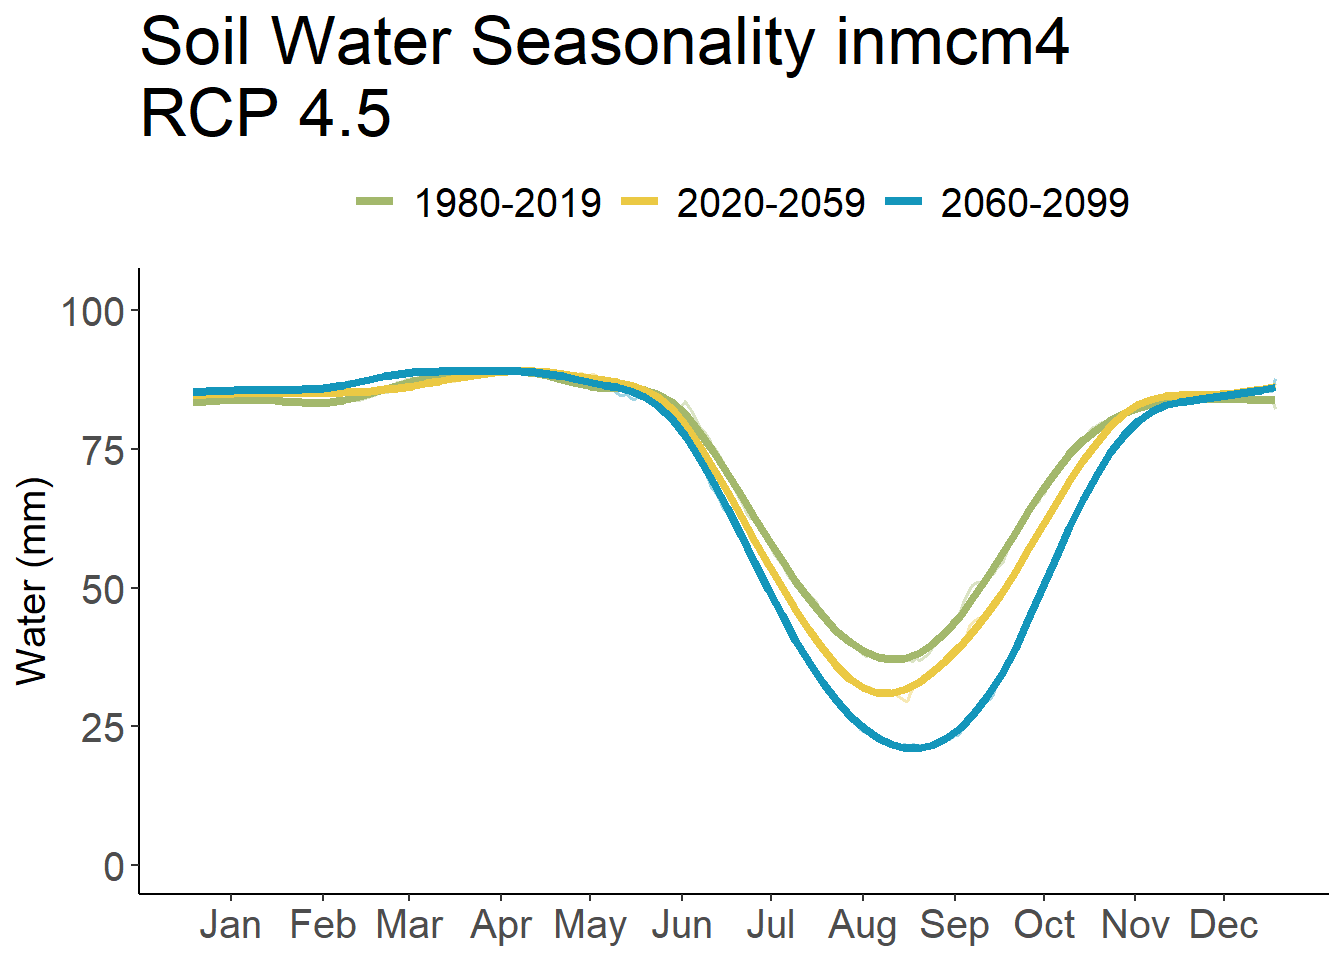
\includegraphics[width=0.5\linewidth]{water_balance_graphs_files/figure-latex/unnamed-chunk-20-1}
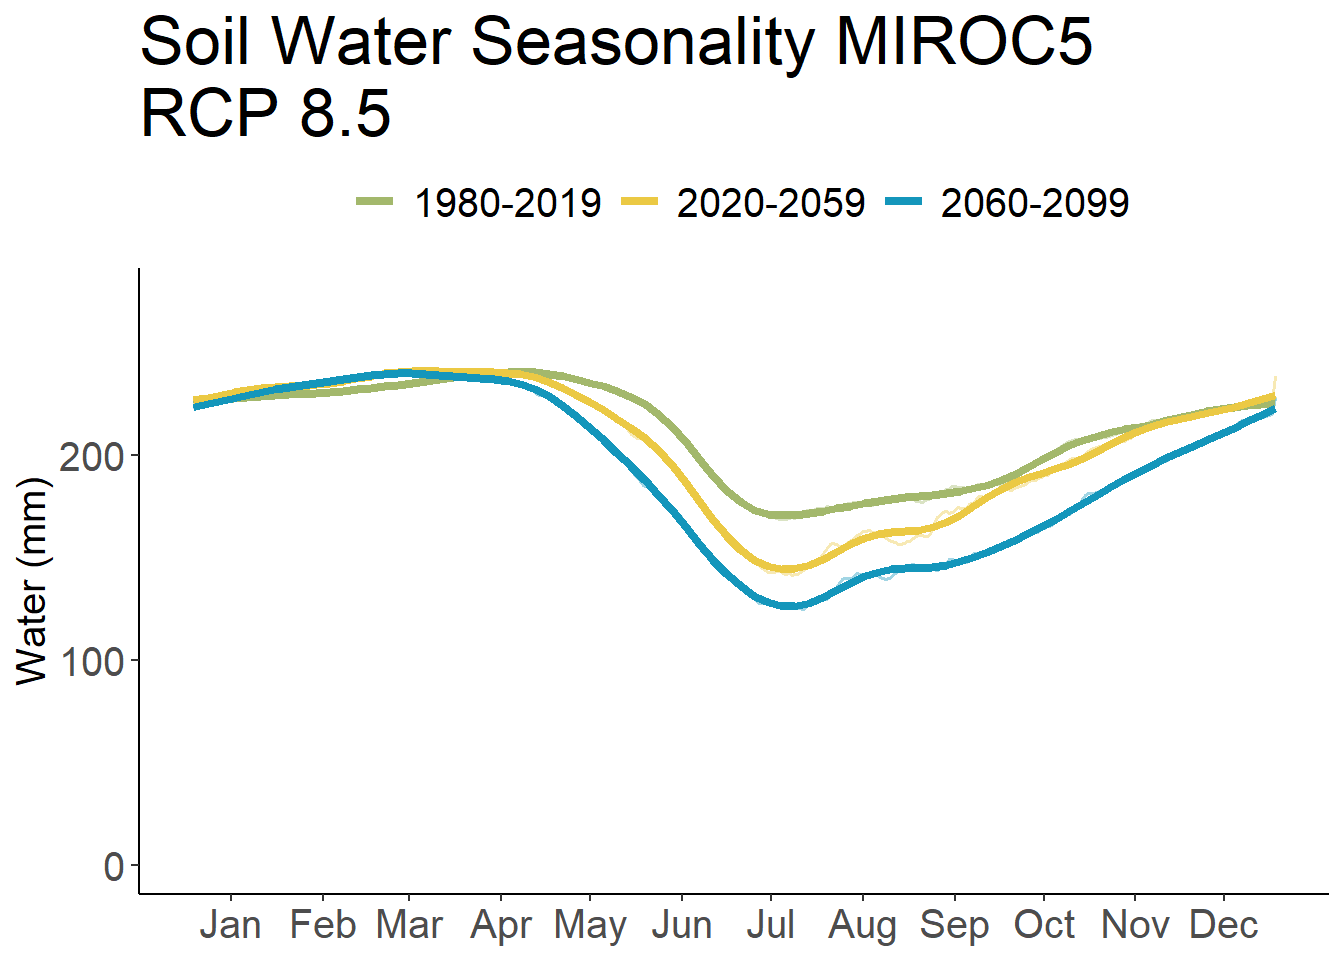
\includegraphics[width=0.5\linewidth]{water_balance_graphs_files/figure-latex/unnamed-chunk-20-2}
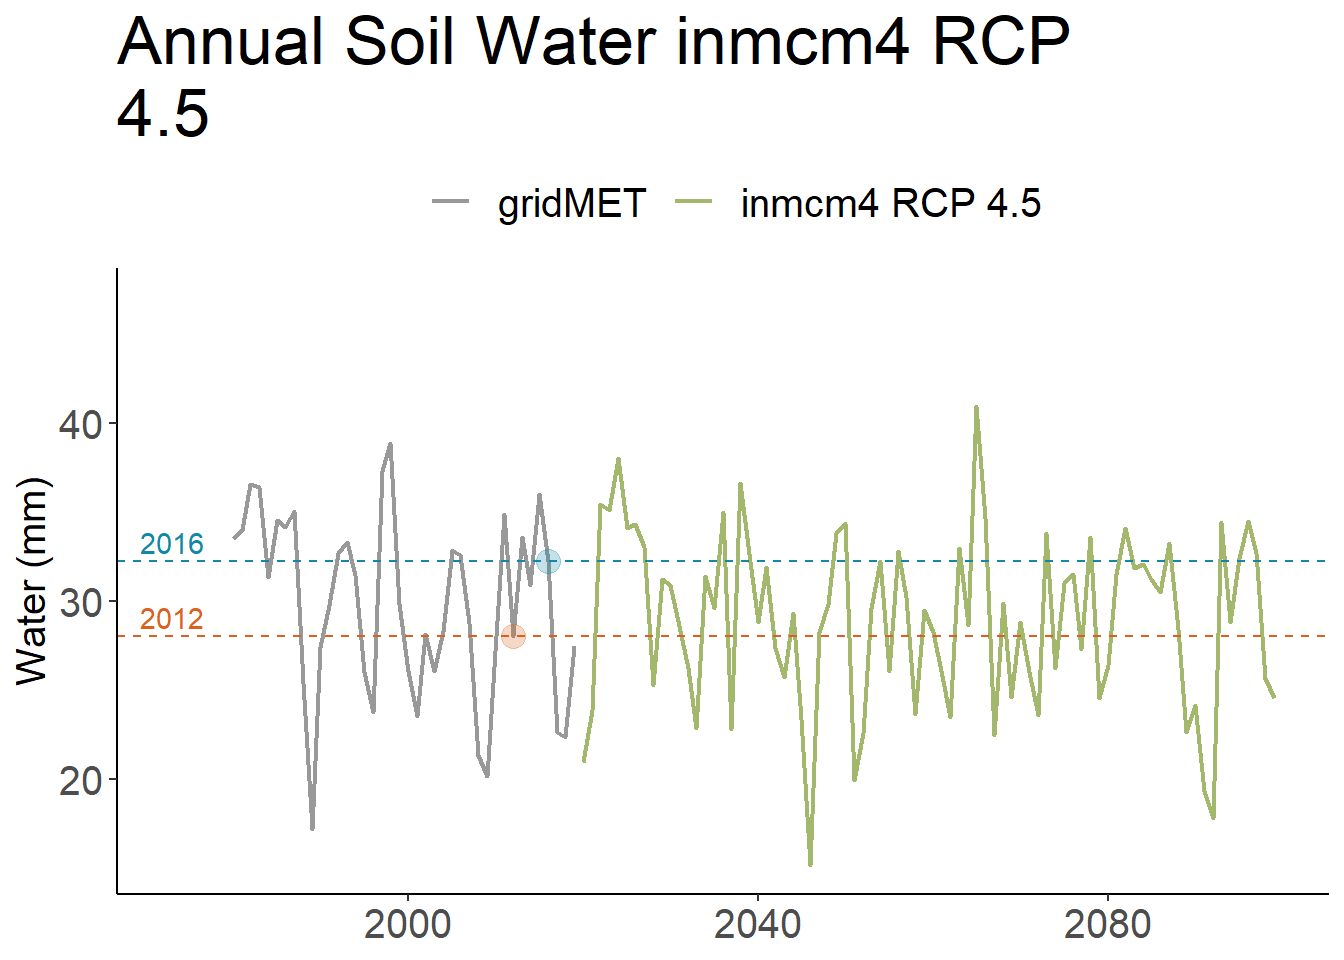
\includegraphics[width=0.5\linewidth]{water_balance_graphs_files/figure-latex/unnamed-chunk-20-3}
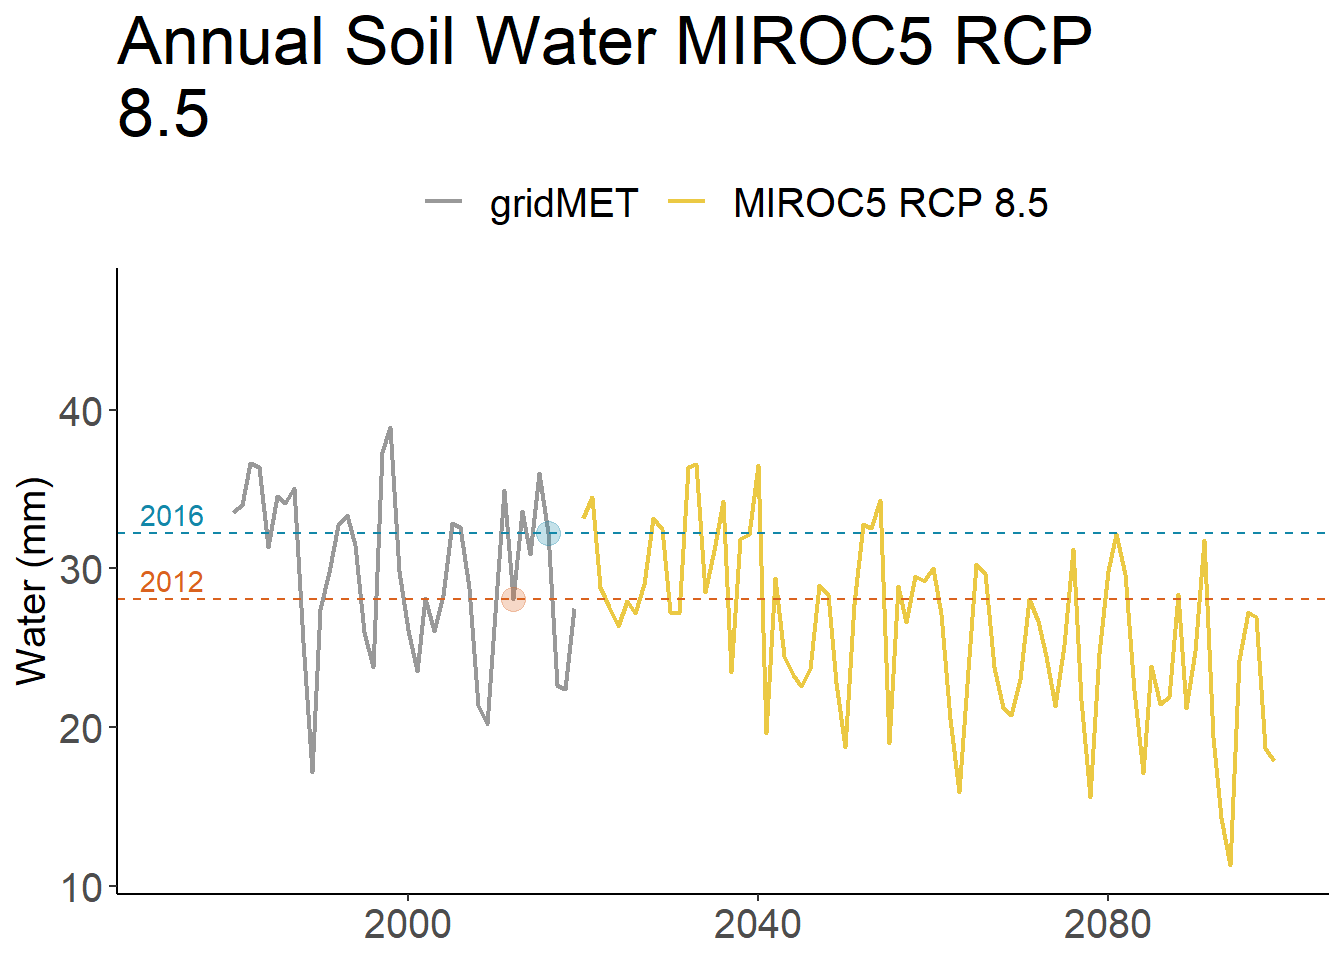
\includegraphics[width=0.5\linewidth]{water_balance_graphs_files/figure-latex/unnamed-chunk-20-4}
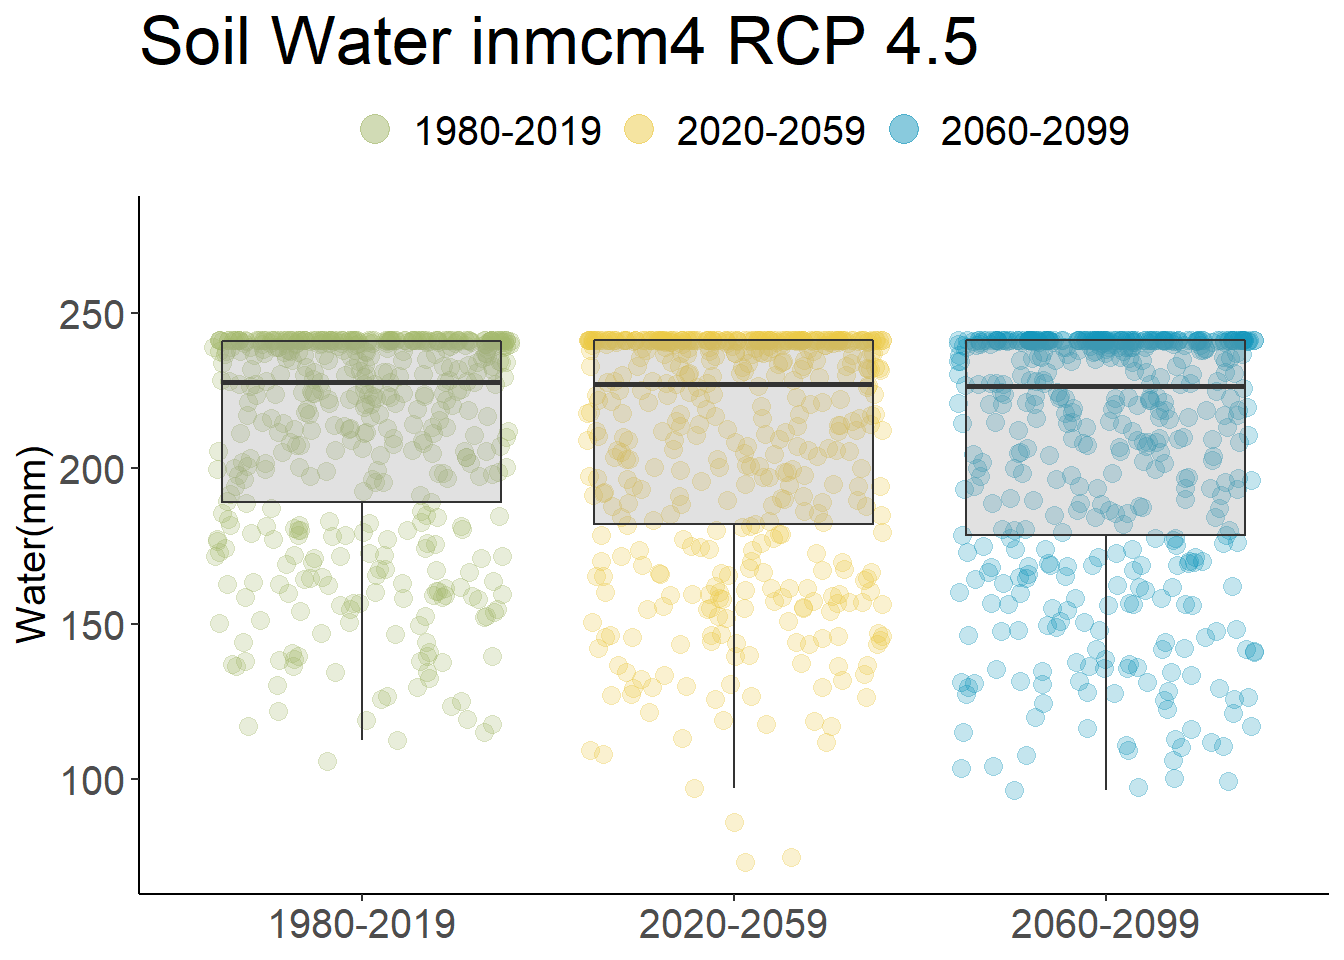
\includegraphics[width=0.5\linewidth]{water_balance_graphs_files/figure-latex/unnamed-chunk-20-5}
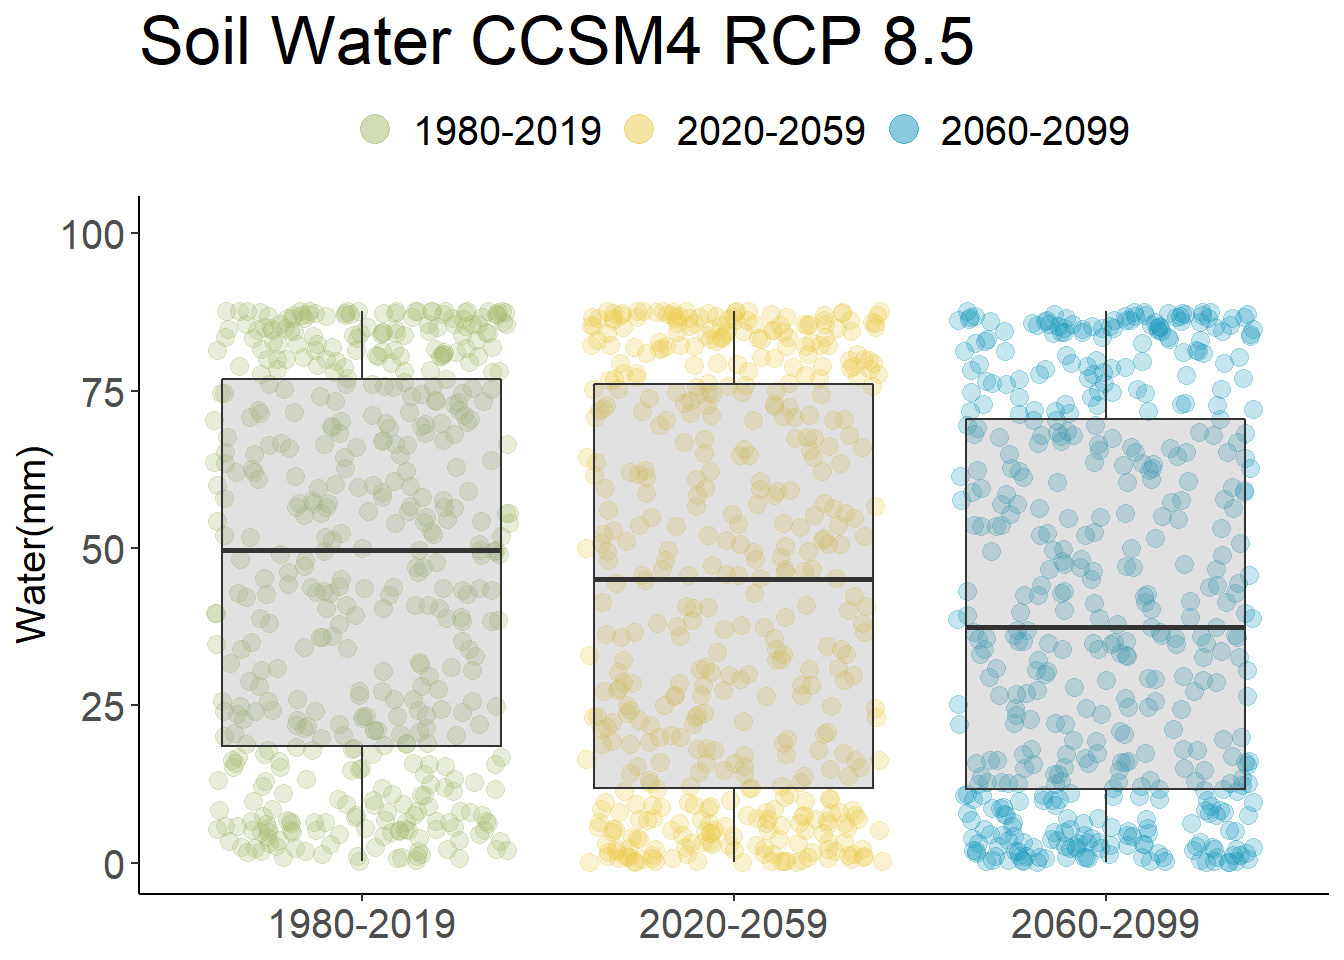
\includegraphics[width=0.5\linewidth]{water_balance_graphs_files/figure-latex/unnamed-chunk-20-6}

\hypertarget{rain}{%
\subsection{Rain}\label{rain}}

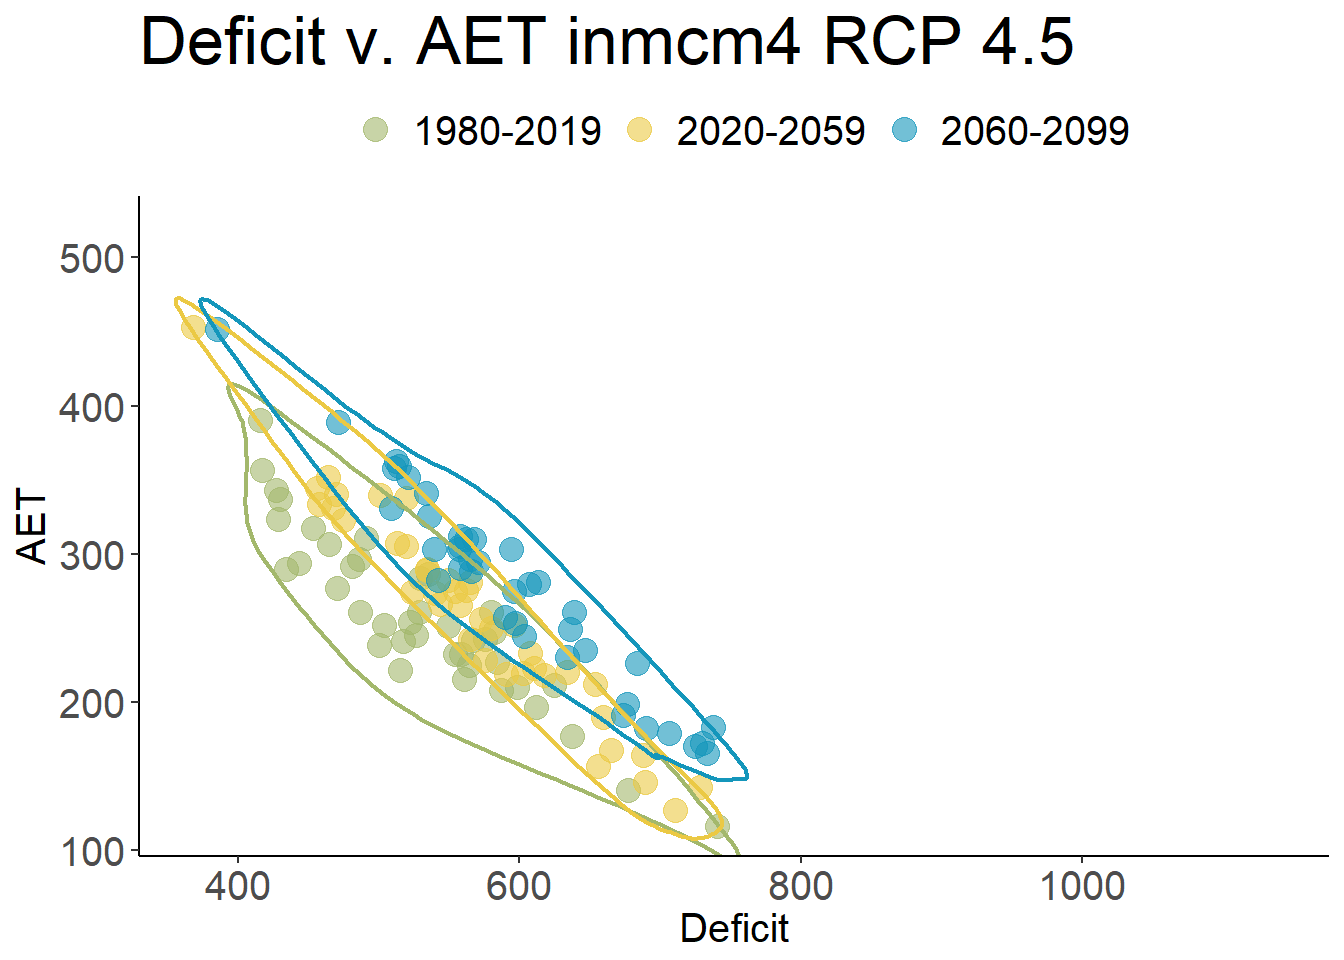
\includegraphics[width=0.5\linewidth]{water_balance_graphs_files/figure-latex/unnamed-chunk-21-1}
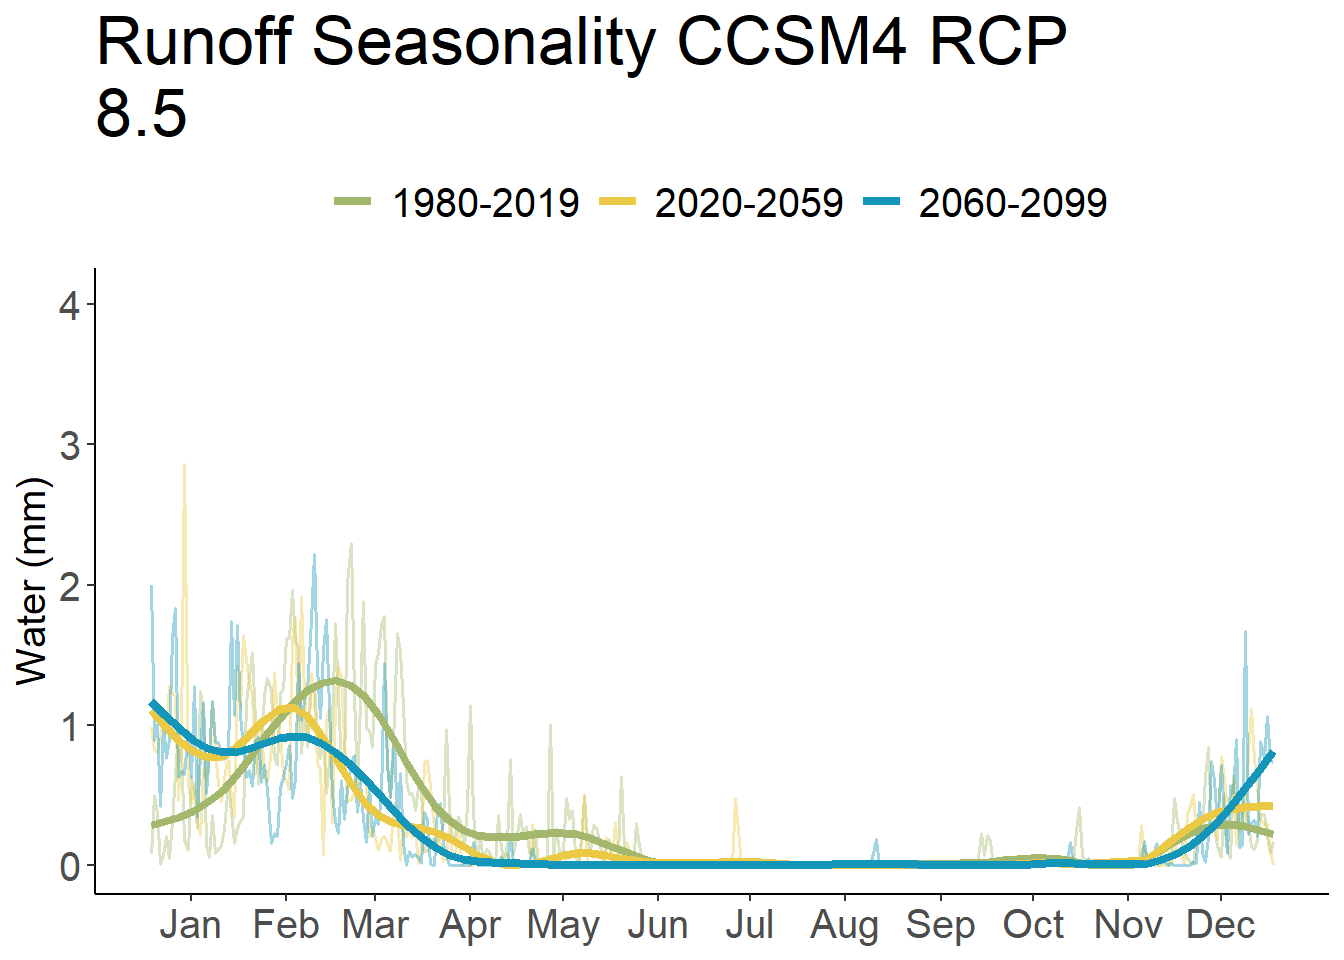
\includegraphics[width=0.5\linewidth]{water_balance_graphs_files/figure-latex/unnamed-chunk-21-2}
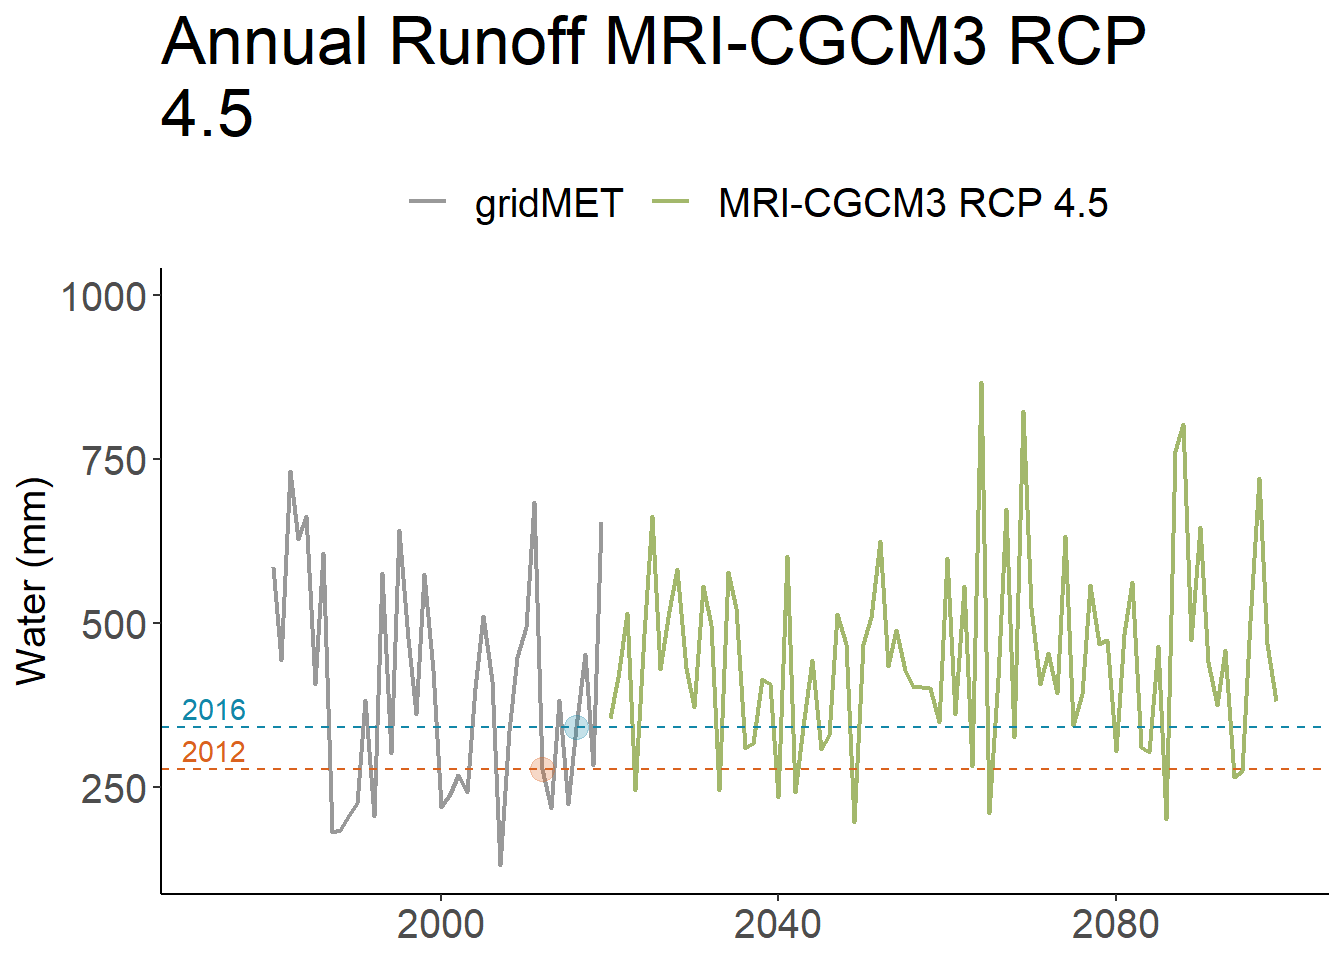
\includegraphics[width=0.5\linewidth]{water_balance_graphs_files/figure-latex/unnamed-chunk-21-3}
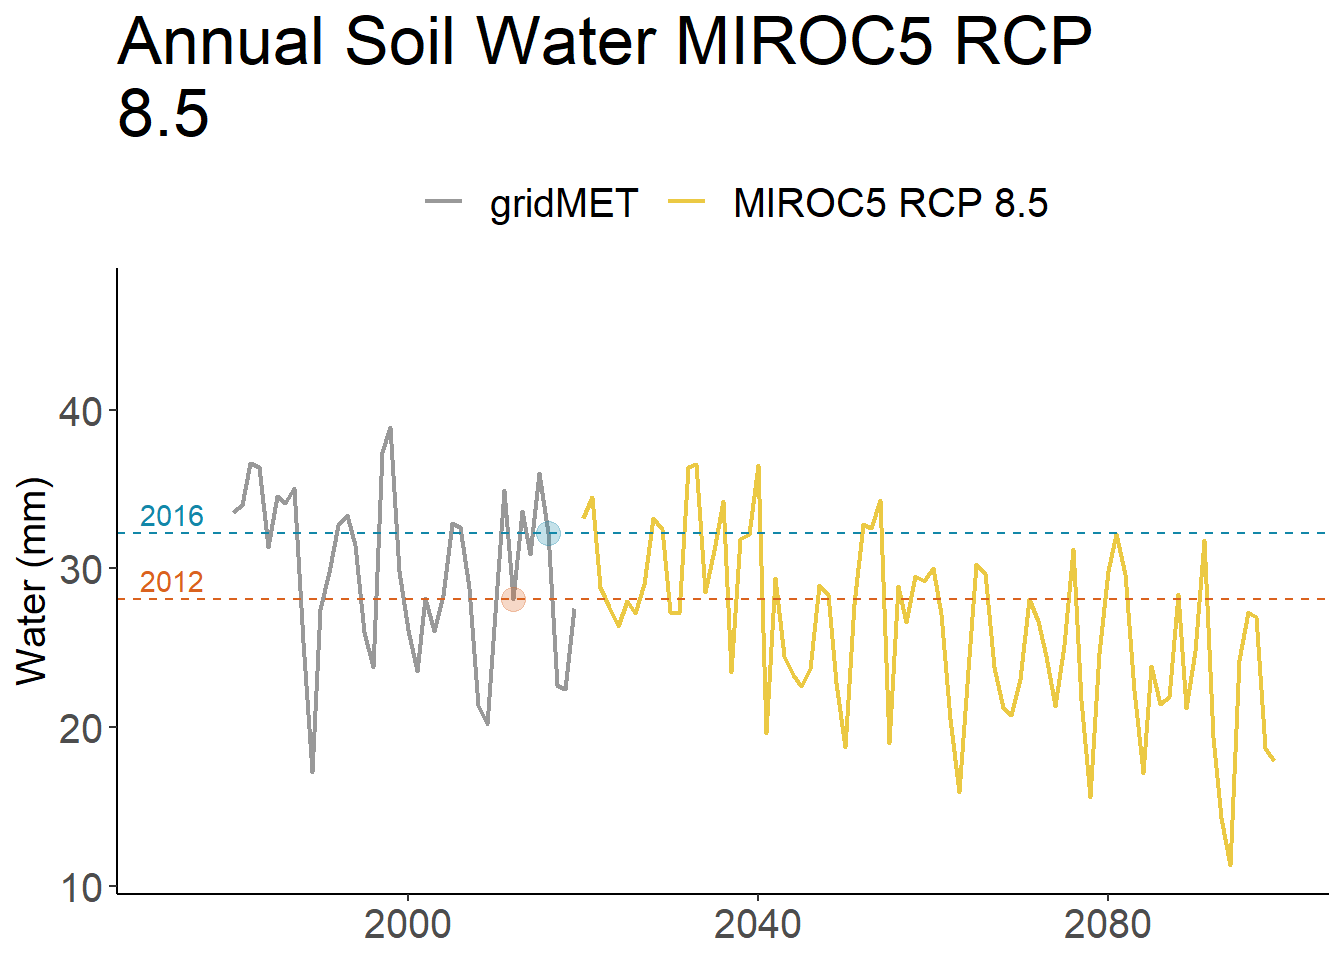
\includegraphics[width=0.5\linewidth]{water_balance_graphs_files/figure-latex/unnamed-chunk-21-4}
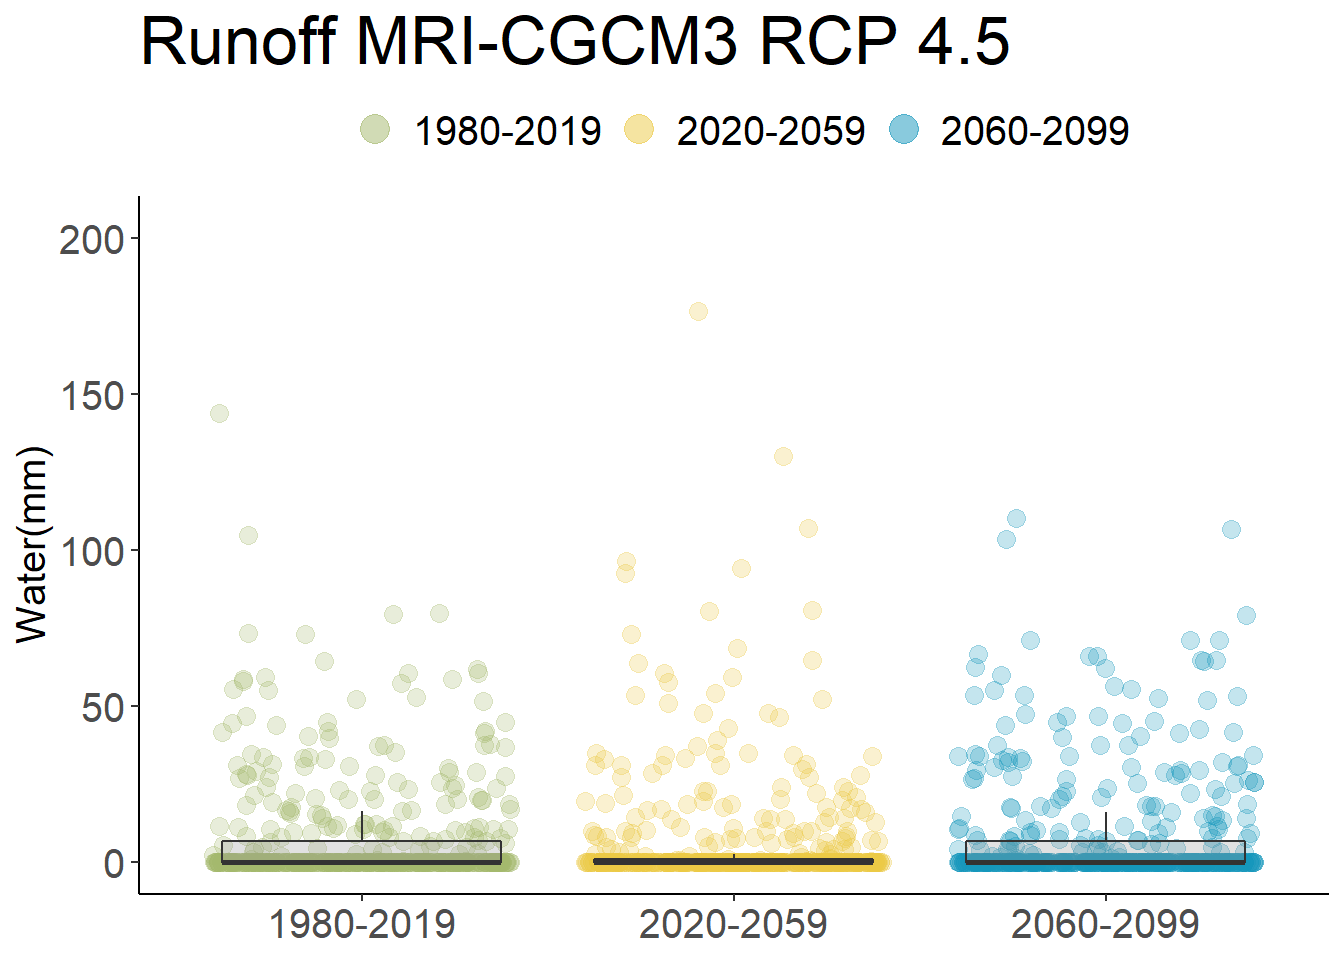
\includegraphics[width=0.5\linewidth]{water_balance_graphs_files/figure-latex/unnamed-chunk-21-5}
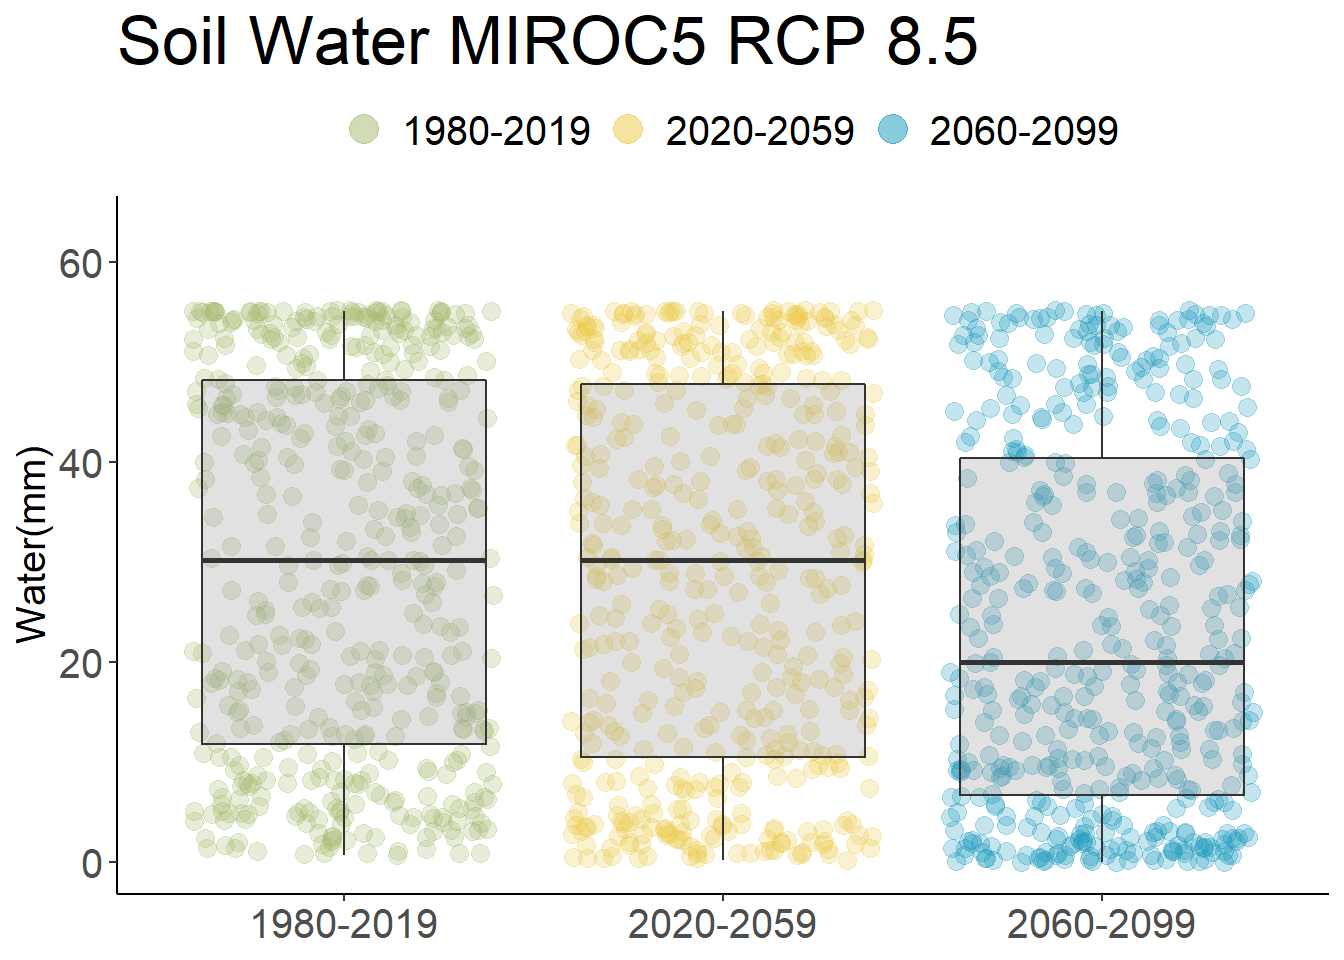
\includegraphics[width=0.5\linewidth]{water_balance_graphs_files/figure-latex/unnamed-chunk-21-6}

\hypertarget{accumulated-snow-water-equivalent-swe}{%
\subsection{Accumulated Snow Water Equivalent
(SWE)}\label{accumulated-snow-water-equivalent-swe}}

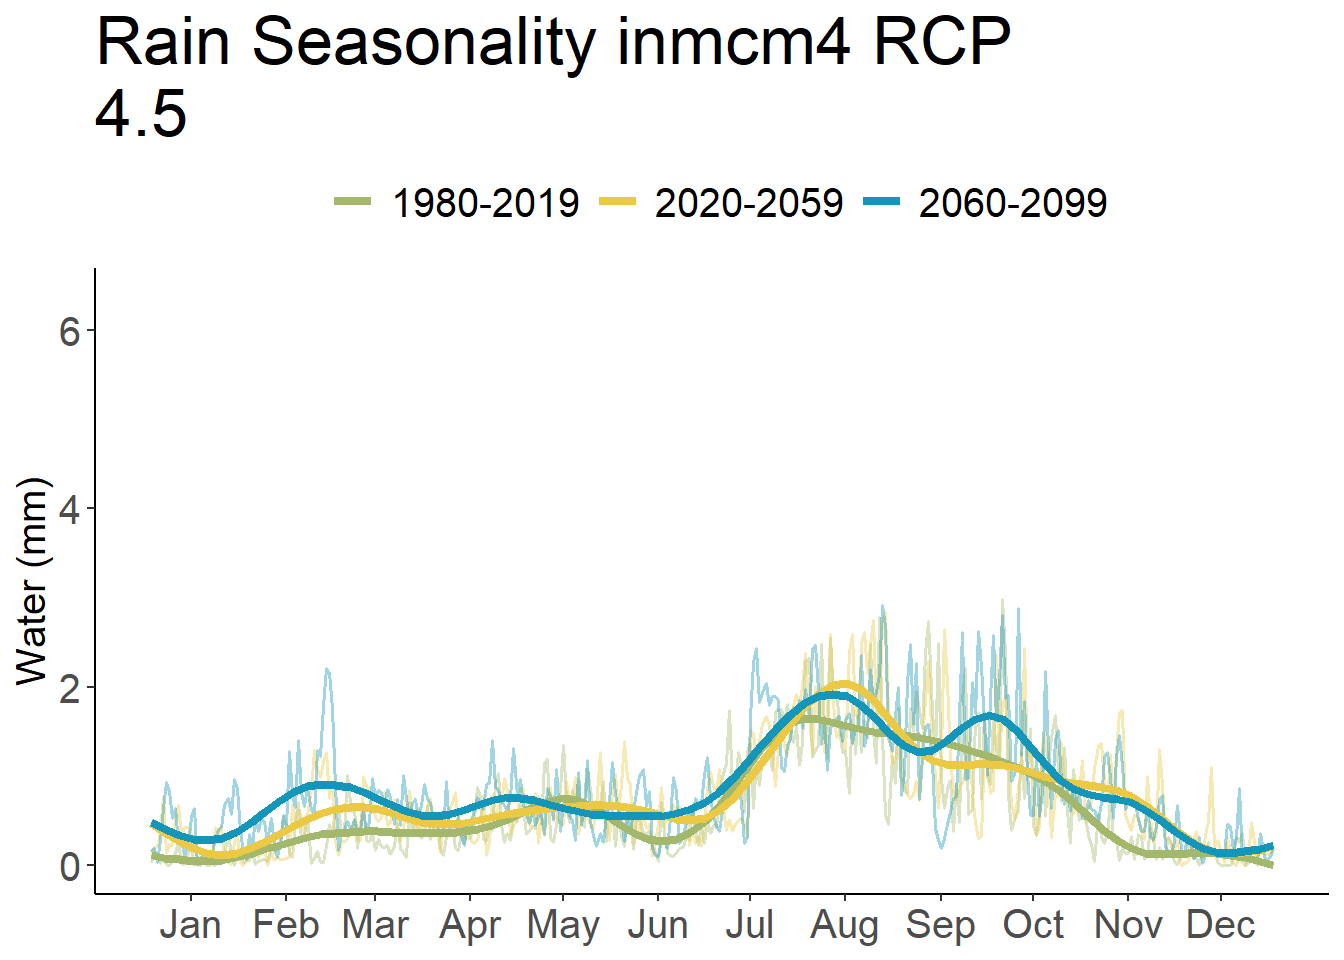
\includegraphics[width=0.5\linewidth]{water_balance_graphs_files/figure-latex/unnamed-chunk-22-1}
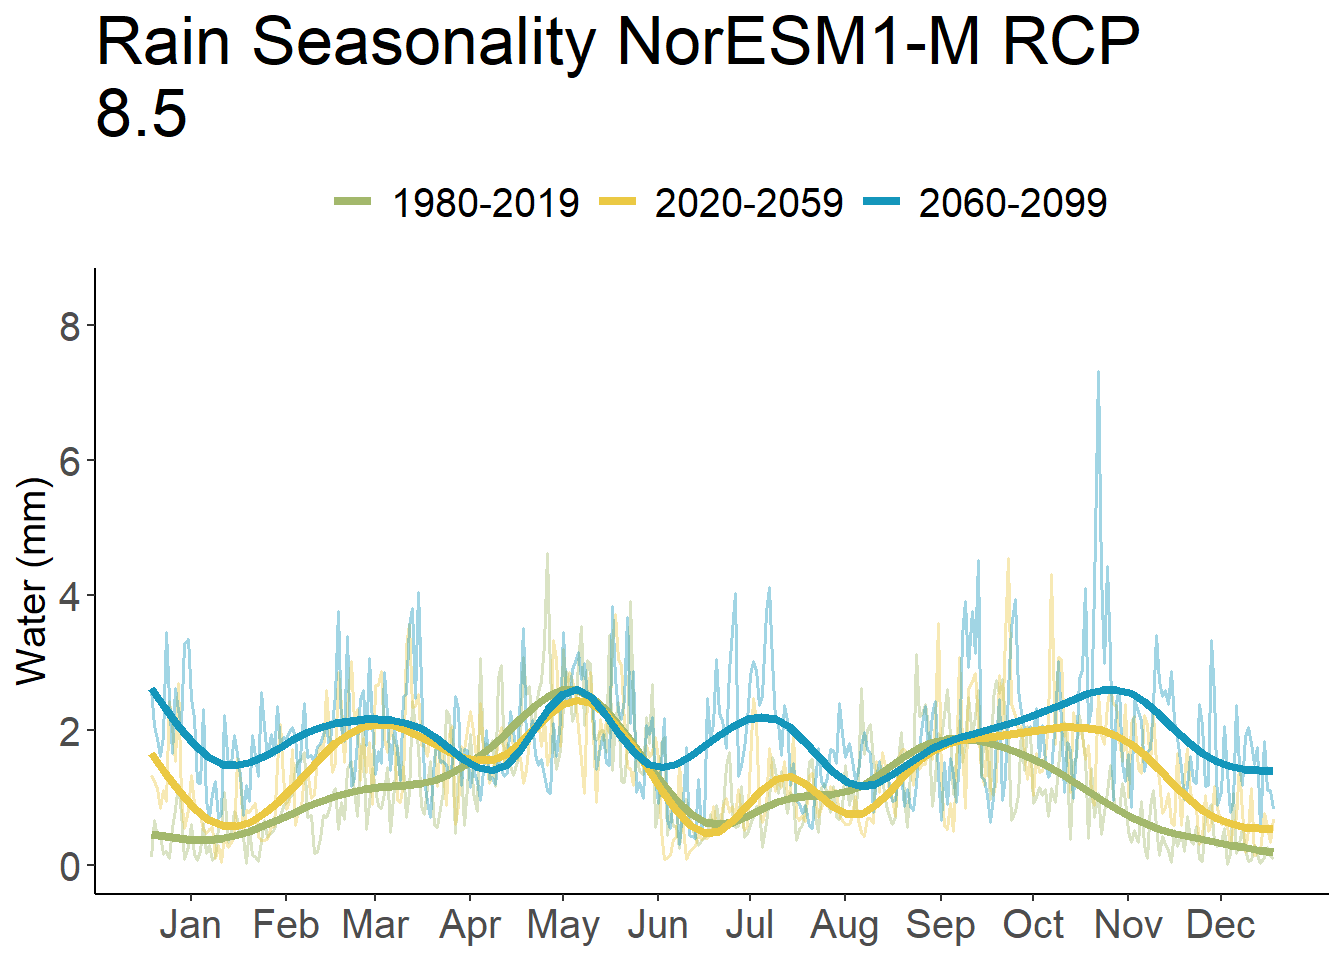
\includegraphics[width=0.5\linewidth]{water_balance_graphs_files/figure-latex/unnamed-chunk-22-2}
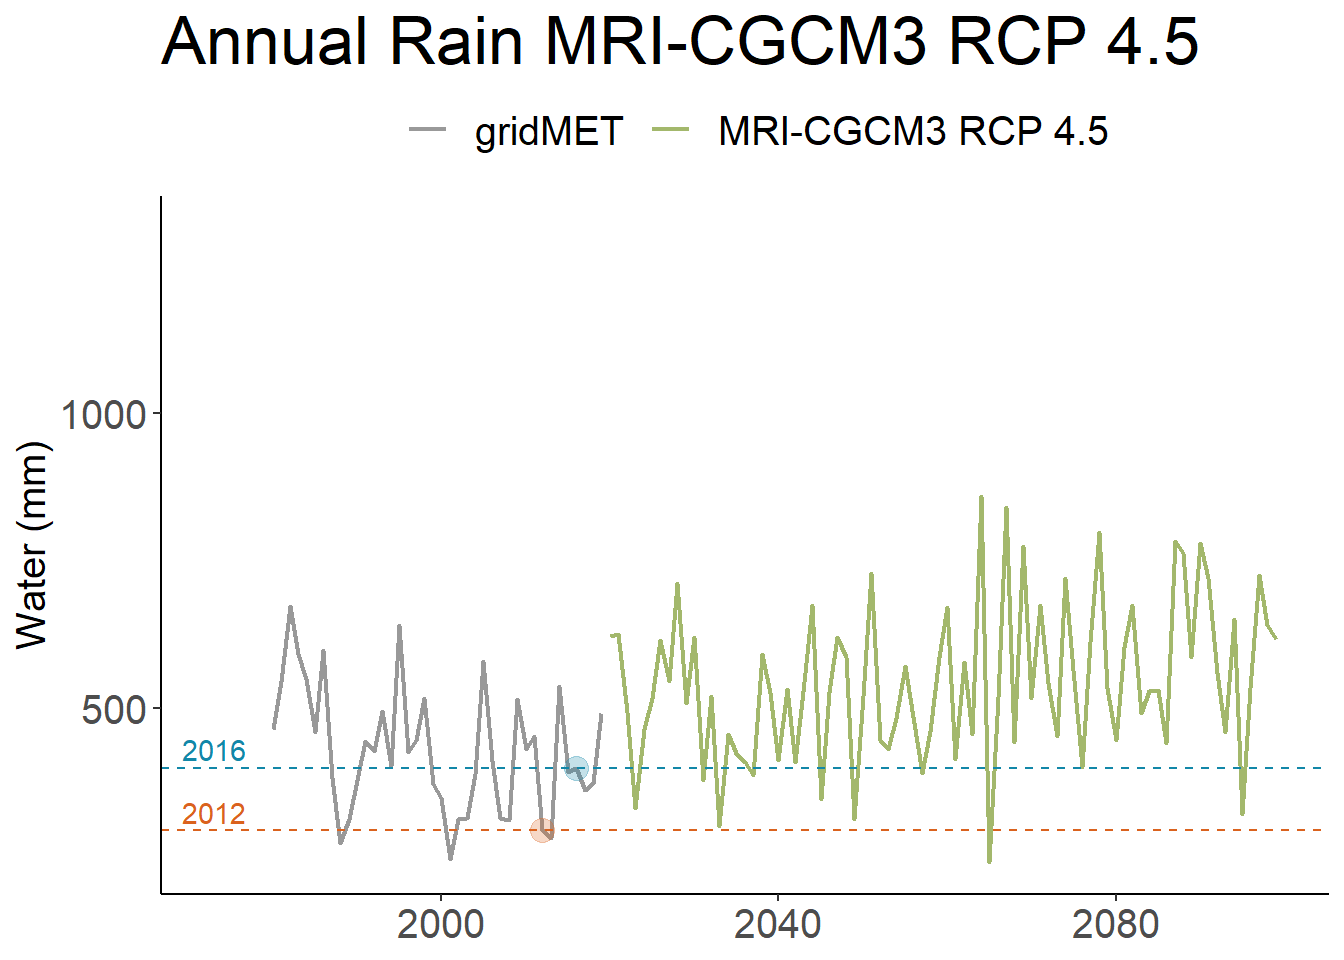
\includegraphics[width=0.5\linewidth]{water_balance_graphs_files/figure-latex/unnamed-chunk-22-3}
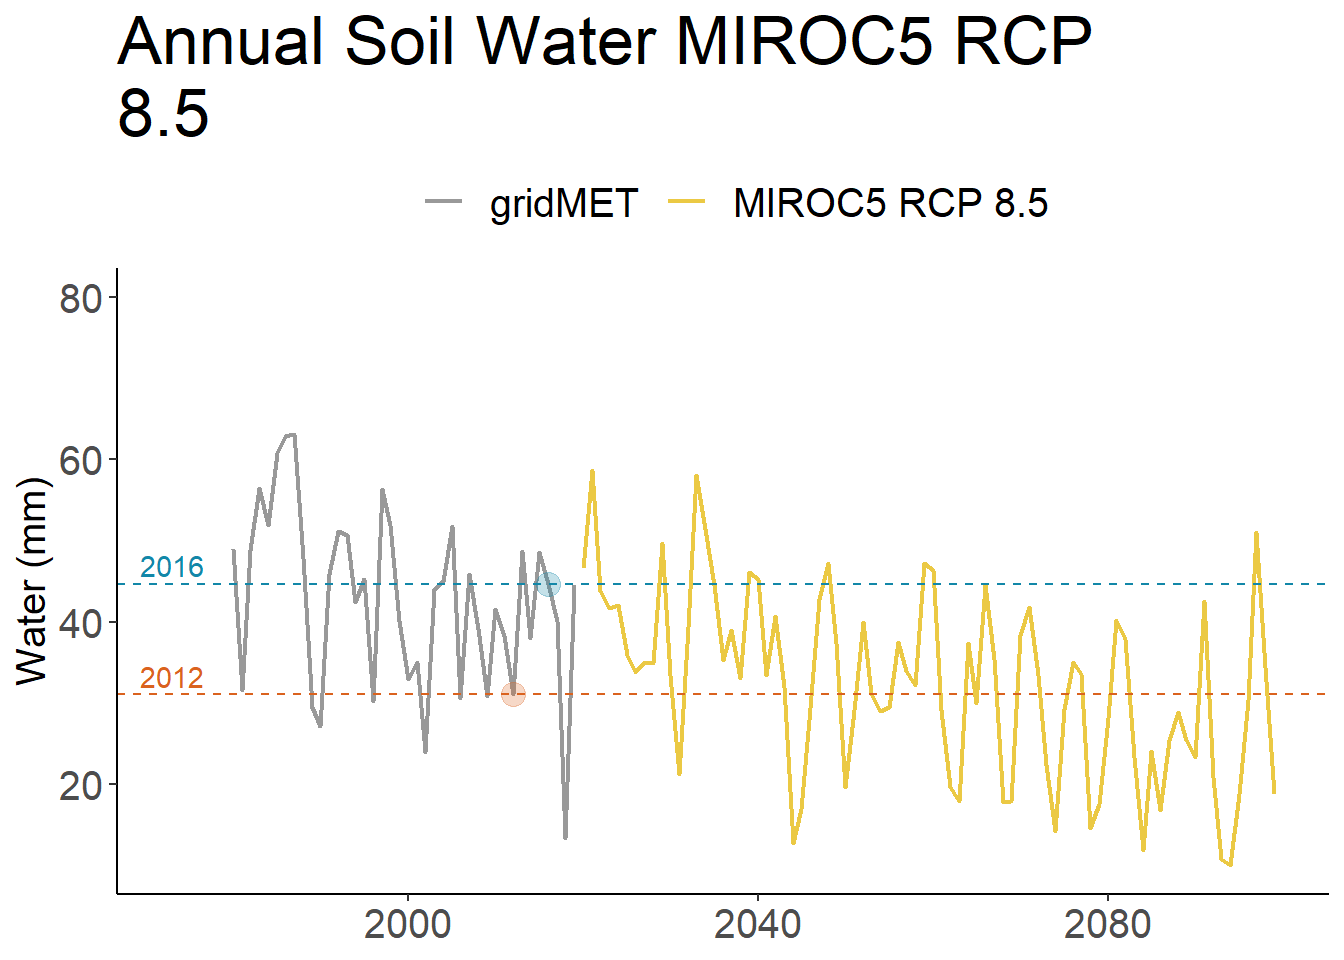
\includegraphics[width=0.5\linewidth]{water_balance_graphs_files/figure-latex/unnamed-chunk-22-4}
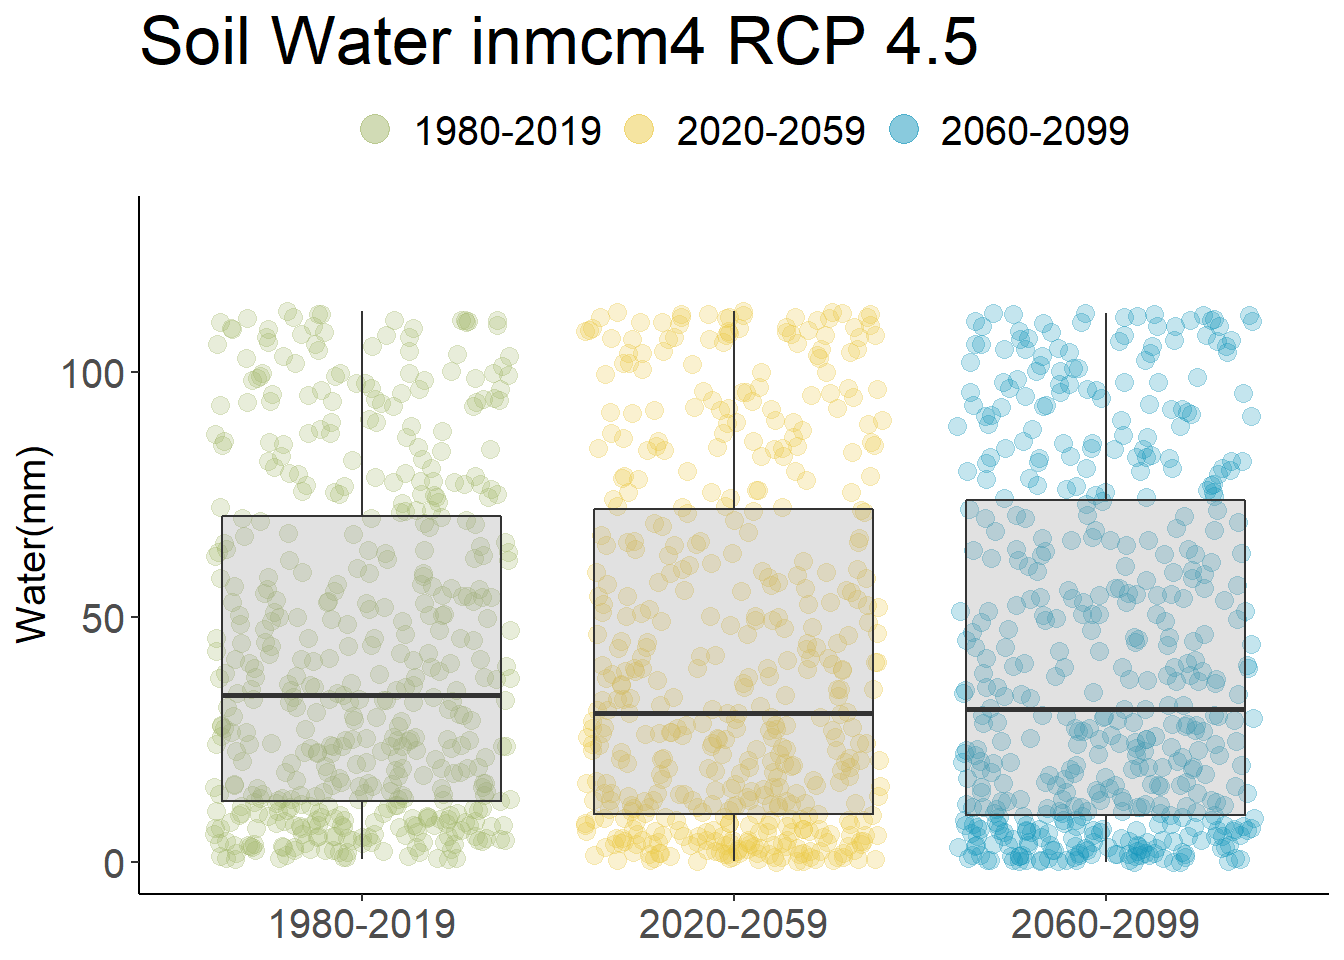
\includegraphics[width=0.5\linewidth]{water_balance_graphs_files/figure-latex/unnamed-chunk-22-5}
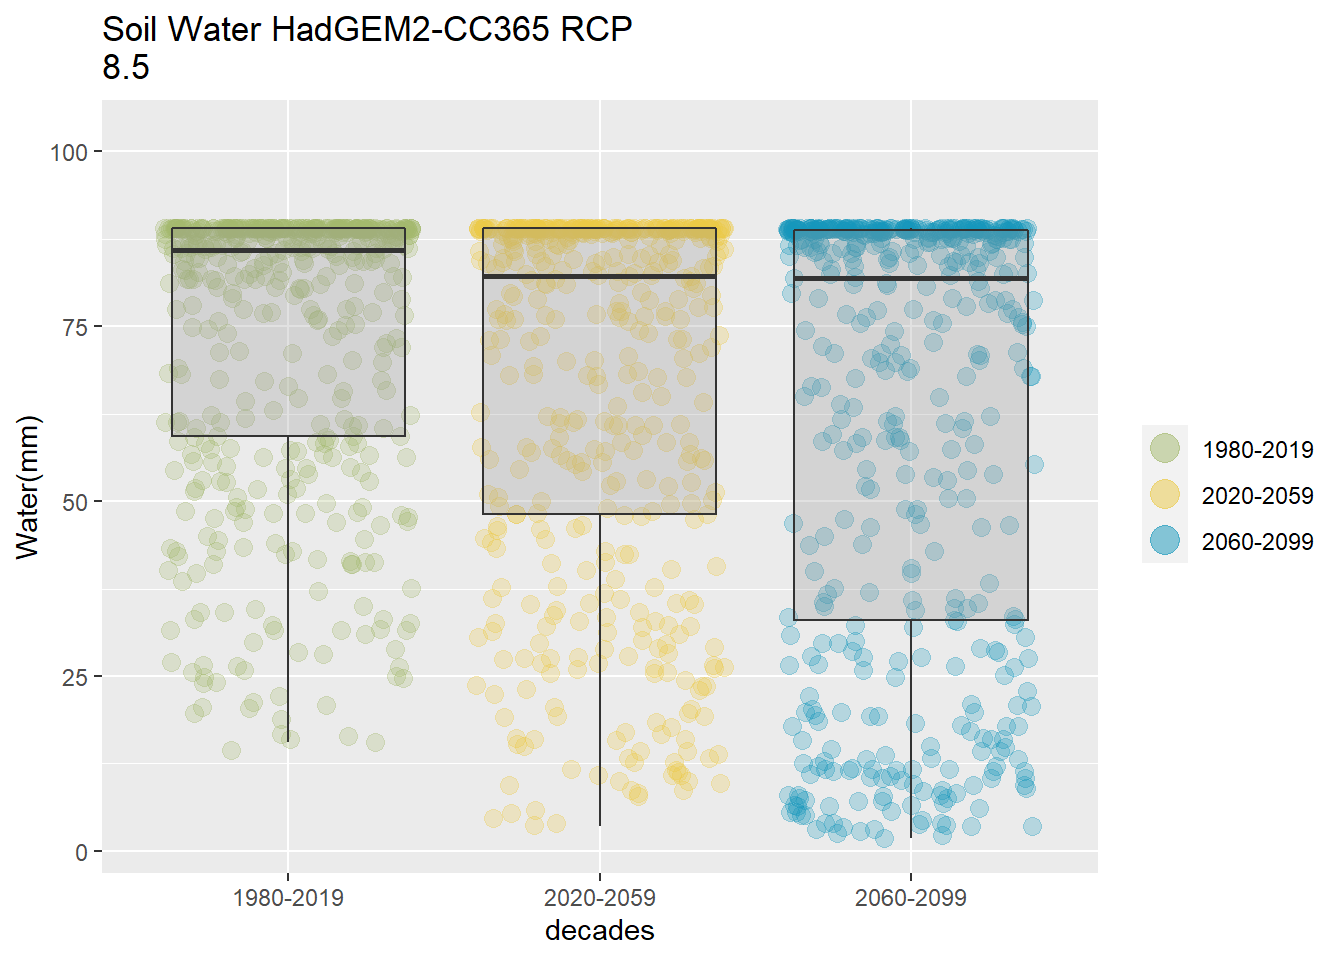
\includegraphics[width=0.5\linewidth]{water_balance_graphs_files/figure-latex/unnamed-chunk-22-6}

\hypertarget{potential-evapotranspiration-pet}{%
\subsection{Potential Evapotranspiration
(PET)}\label{potential-evapotranspiration-pet}}

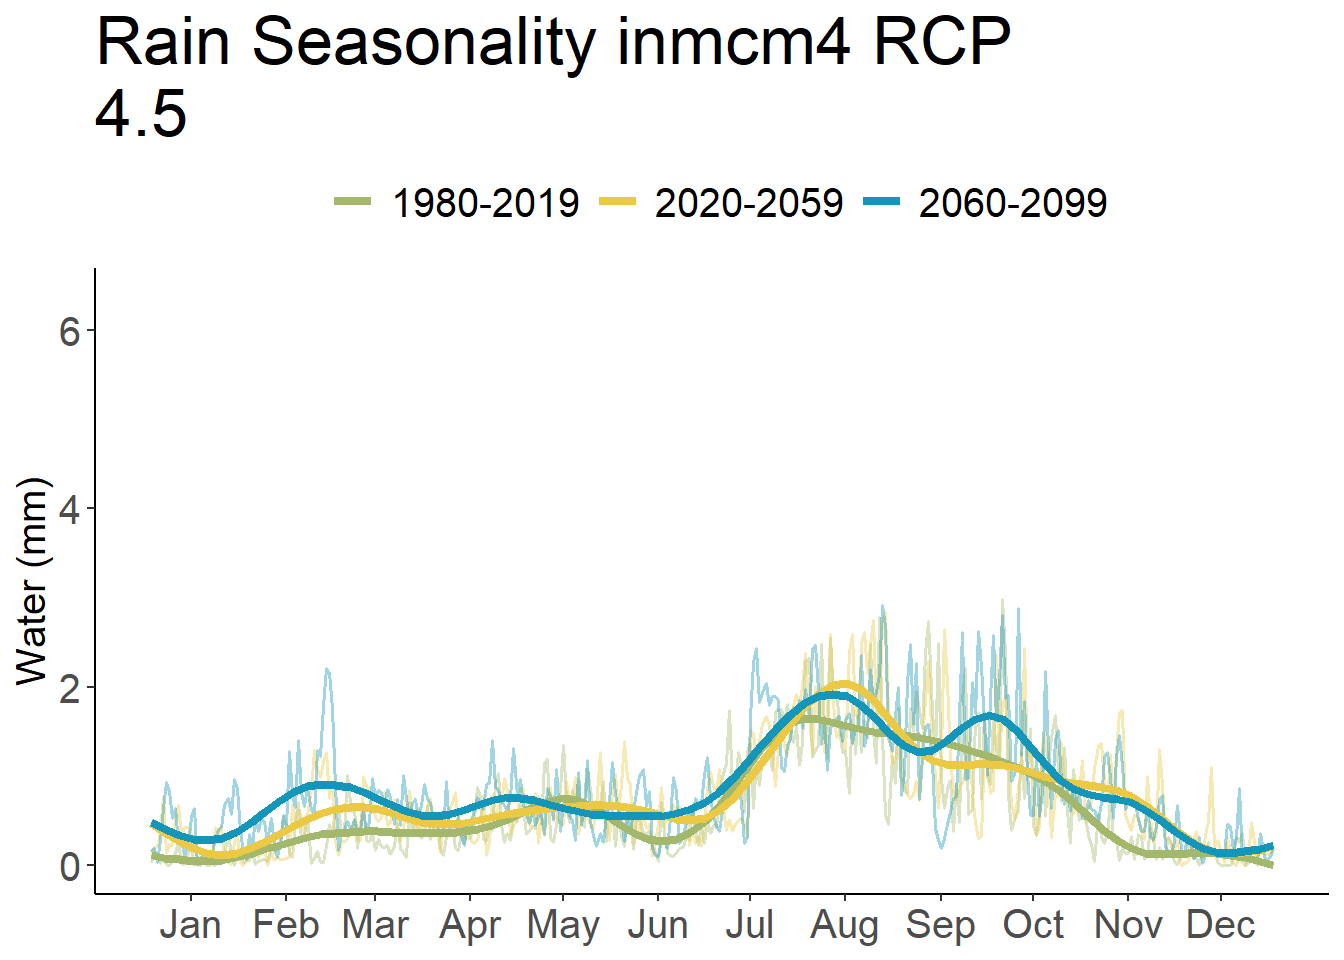
\includegraphics[width=0.5\linewidth]{water_balance_graphs_files/figure-latex/unnamed-chunk-23-1}
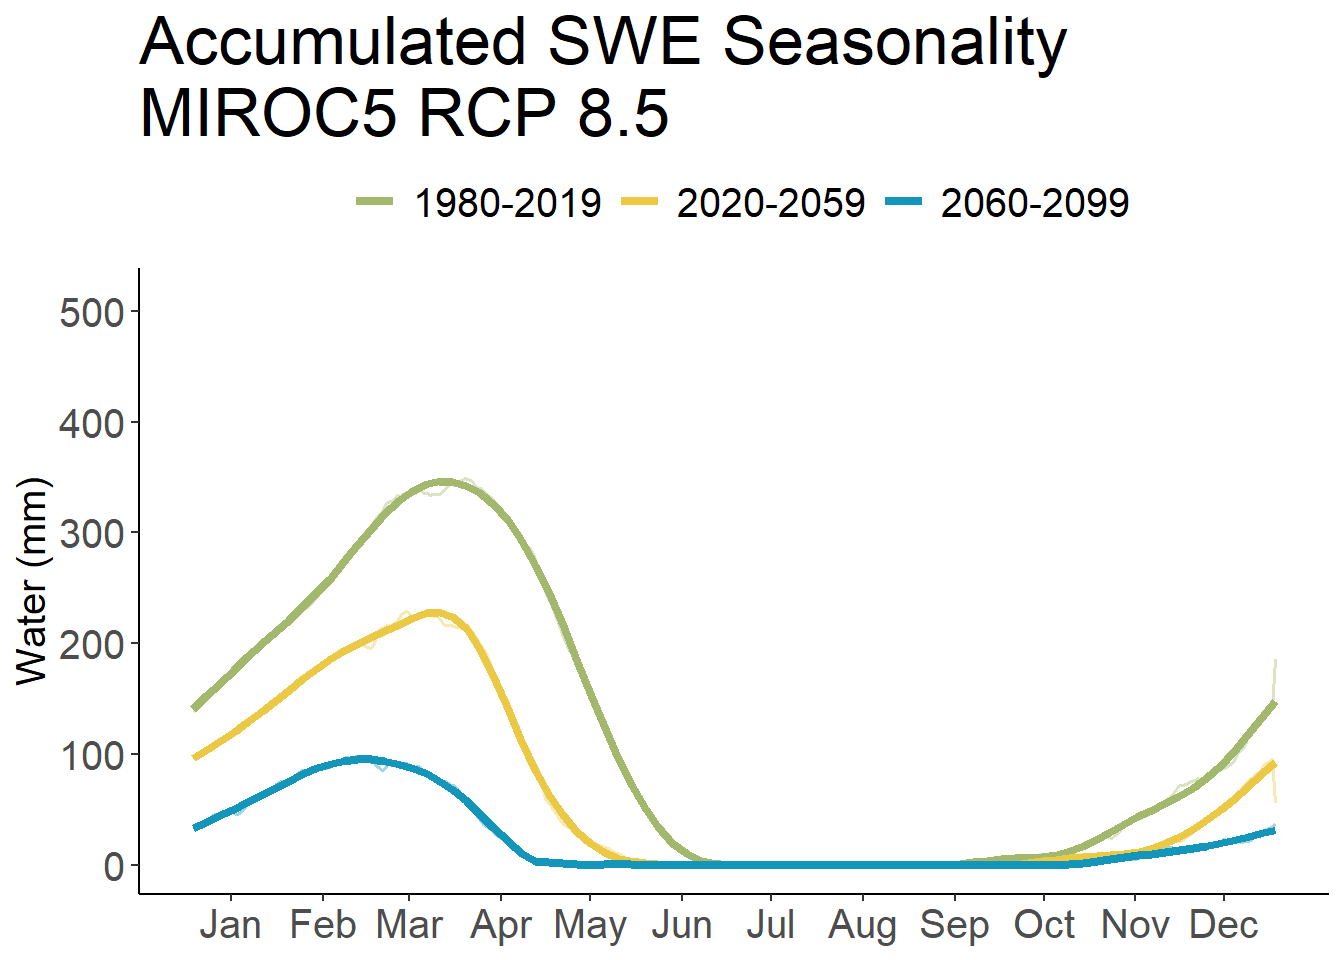
\includegraphics[width=0.5\linewidth]{water_balance_graphs_files/figure-latex/unnamed-chunk-23-2}
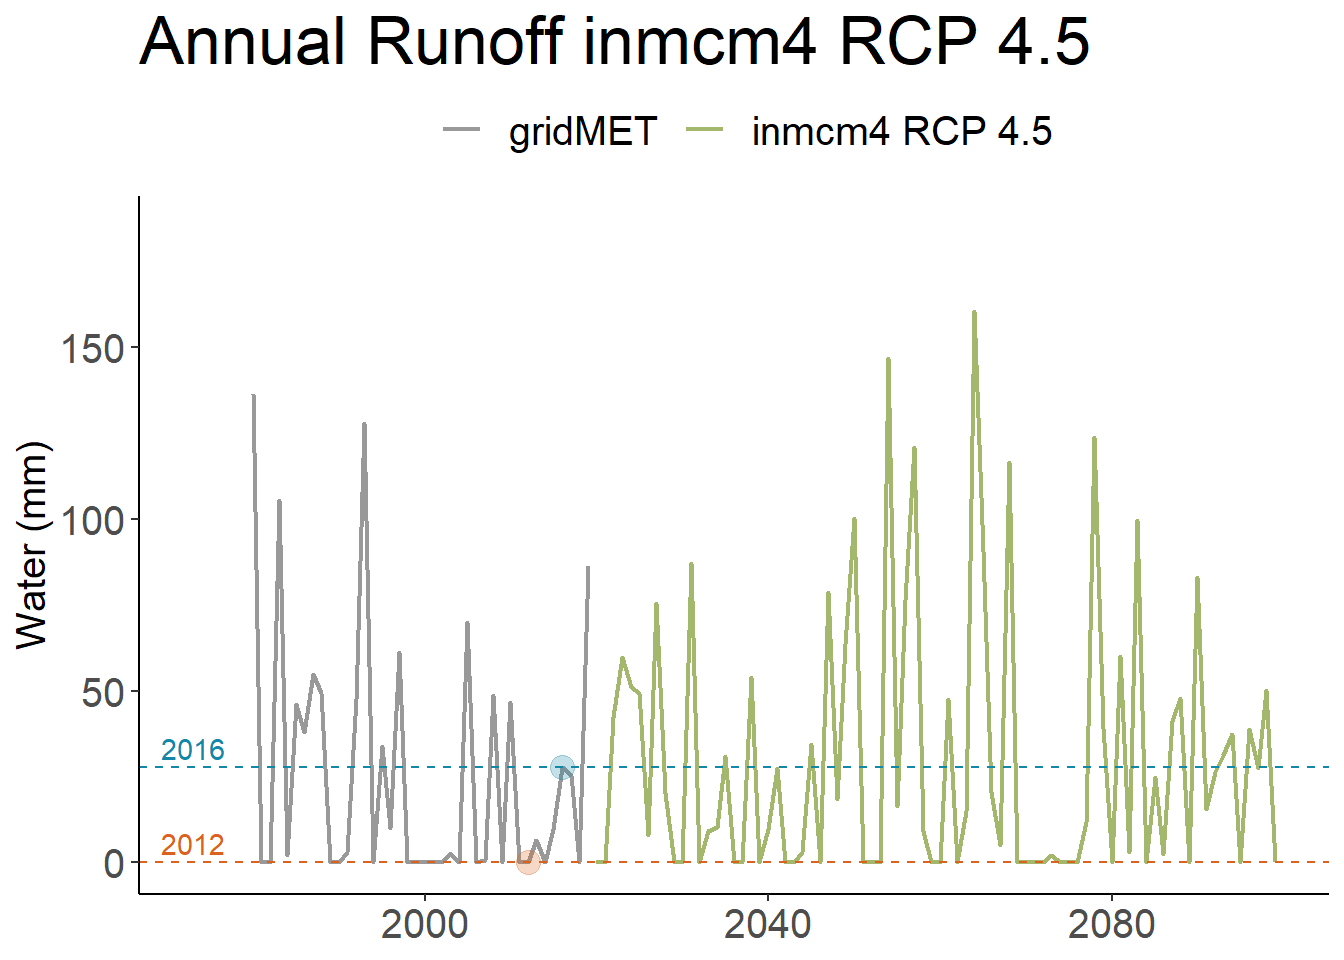
\includegraphics[width=0.5\linewidth]{water_balance_graphs_files/figure-latex/unnamed-chunk-23-3}
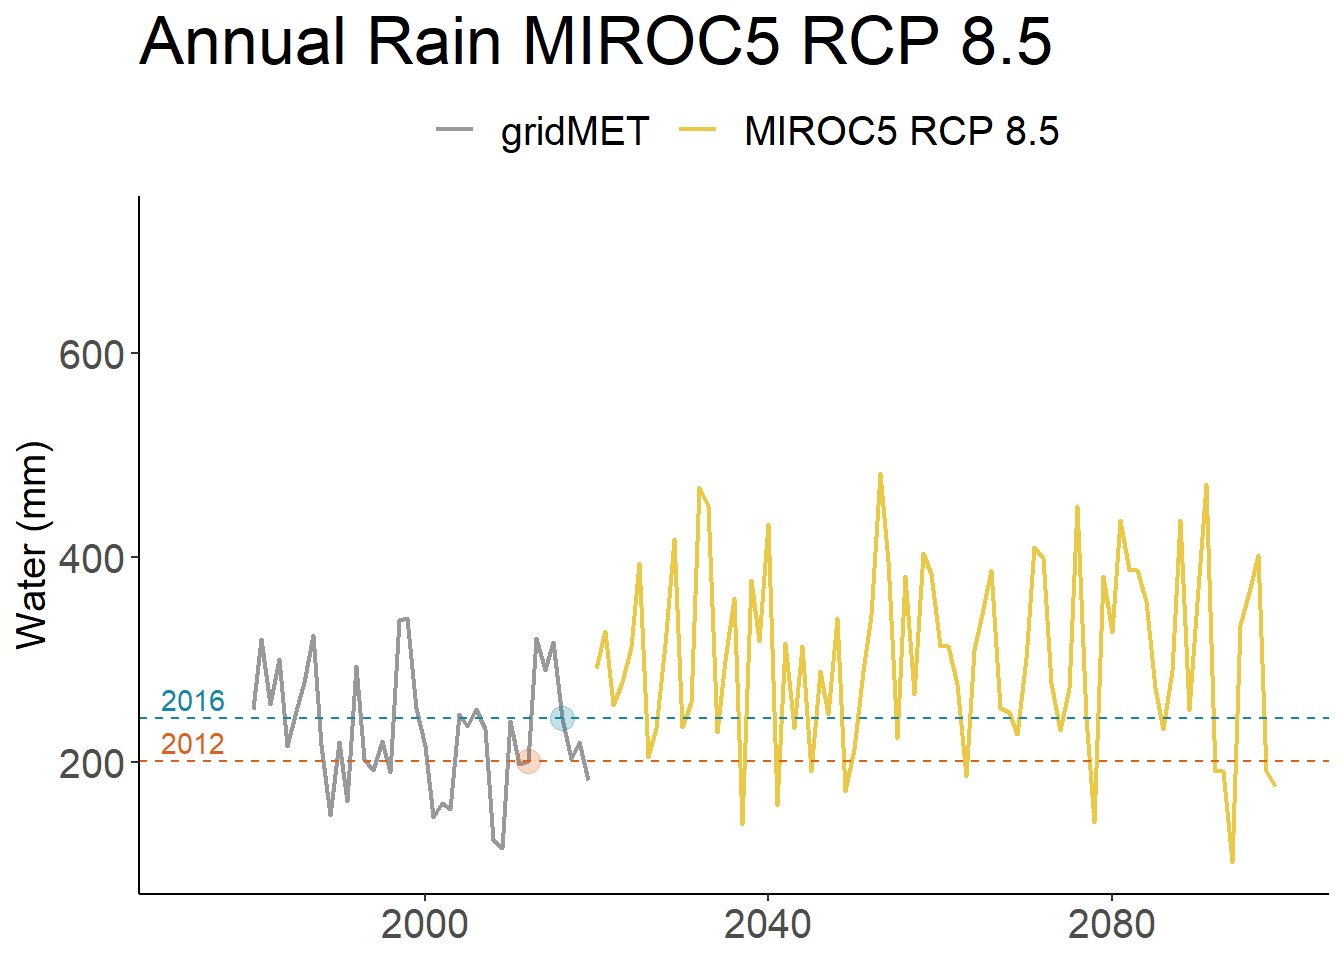
\includegraphics[width=0.5\linewidth]{water_balance_graphs_files/figure-latex/unnamed-chunk-23-4}

\hypertarget{actual-evapotranspiration-aet}{%
\subsection{Actual Evapotranspiration
(AET)}\label{actual-evapotranspiration-aet}}

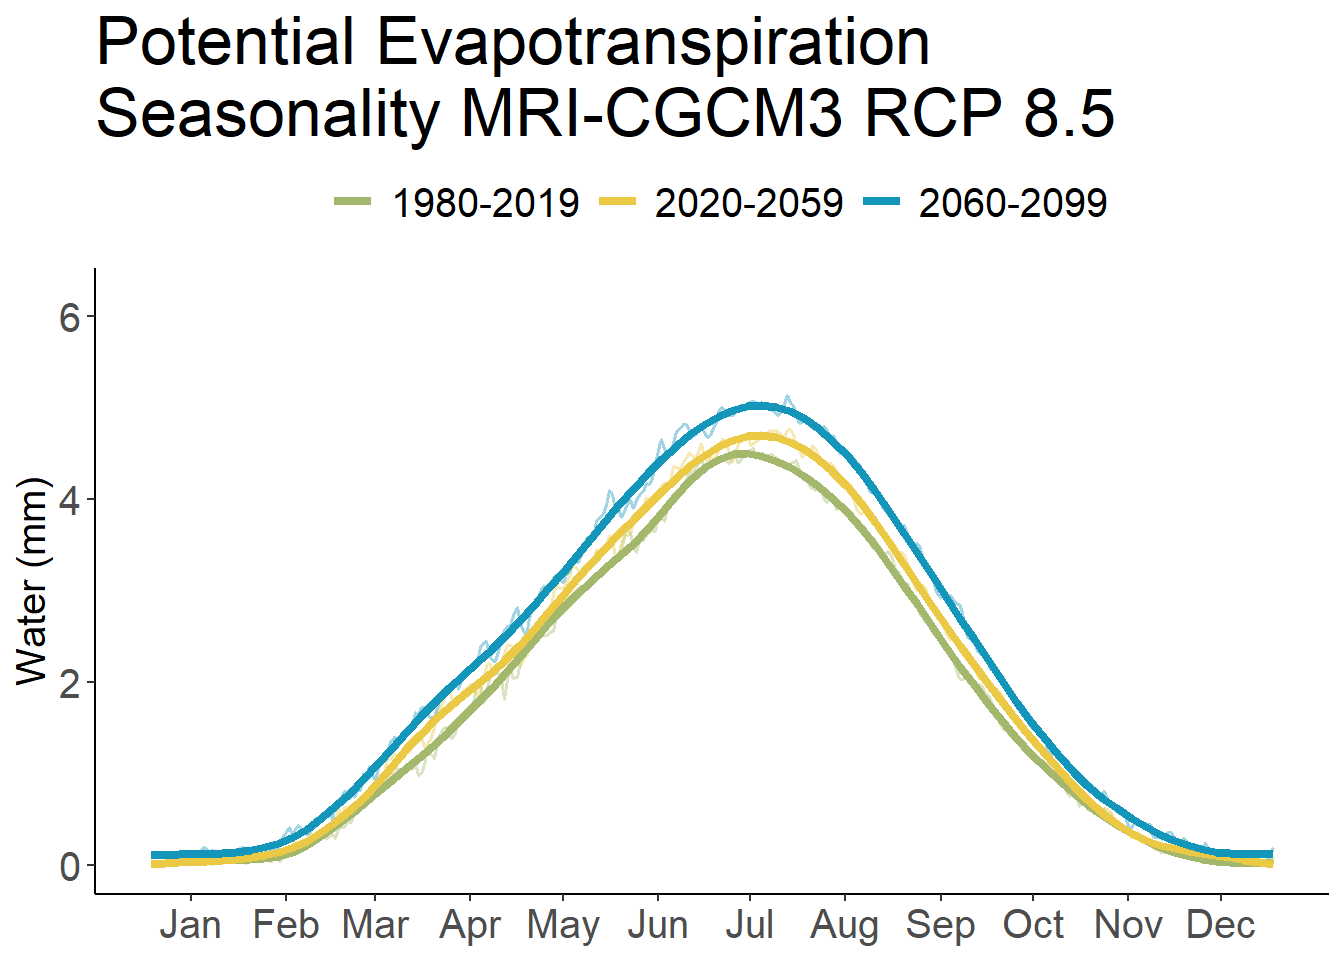
\includegraphics[width=0.5\linewidth]{water_balance_graphs_files/figure-latex/unnamed-chunk-24-1}
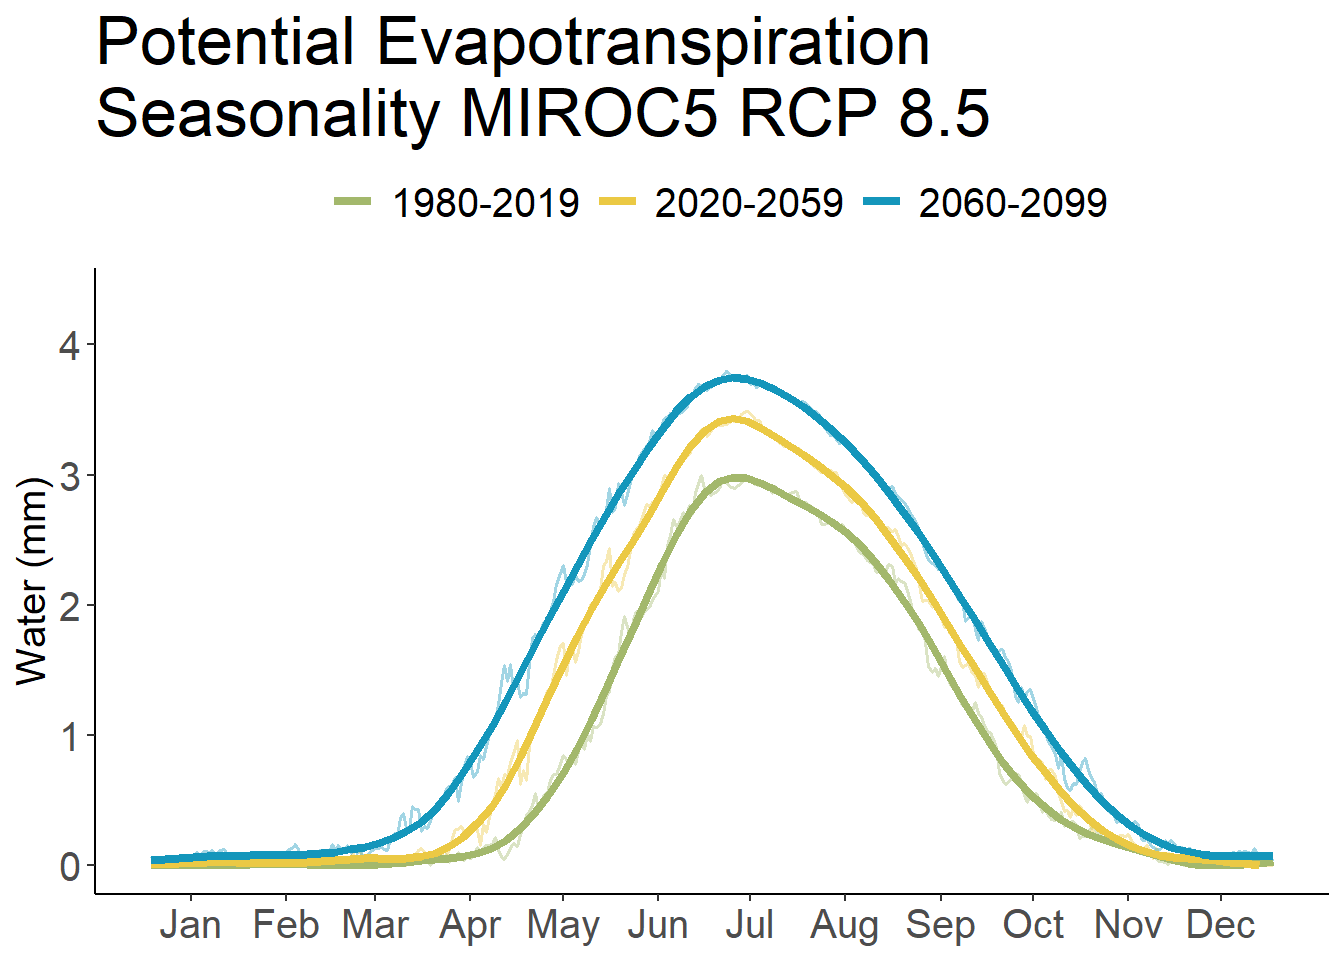
\includegraphics[width=0.5\linewidth]{water_balance_graphs_files/figure-latex/unnamed-chunk-24-2}
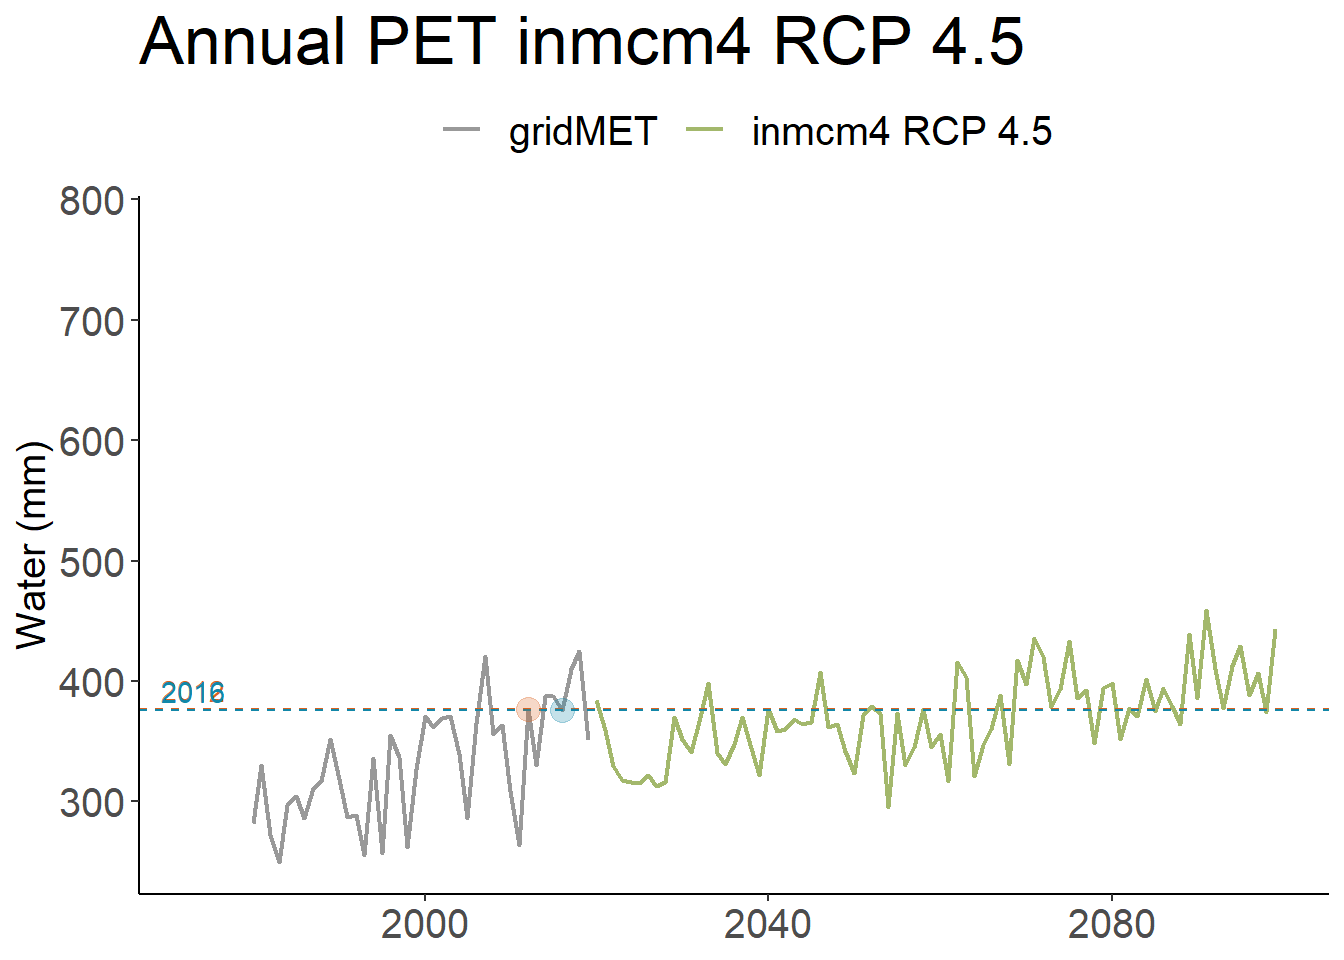
\includegraphics[width=0.5\linewidth]{water_balance_graphs_files/figure-latex/unnamed-chunk-24-3}
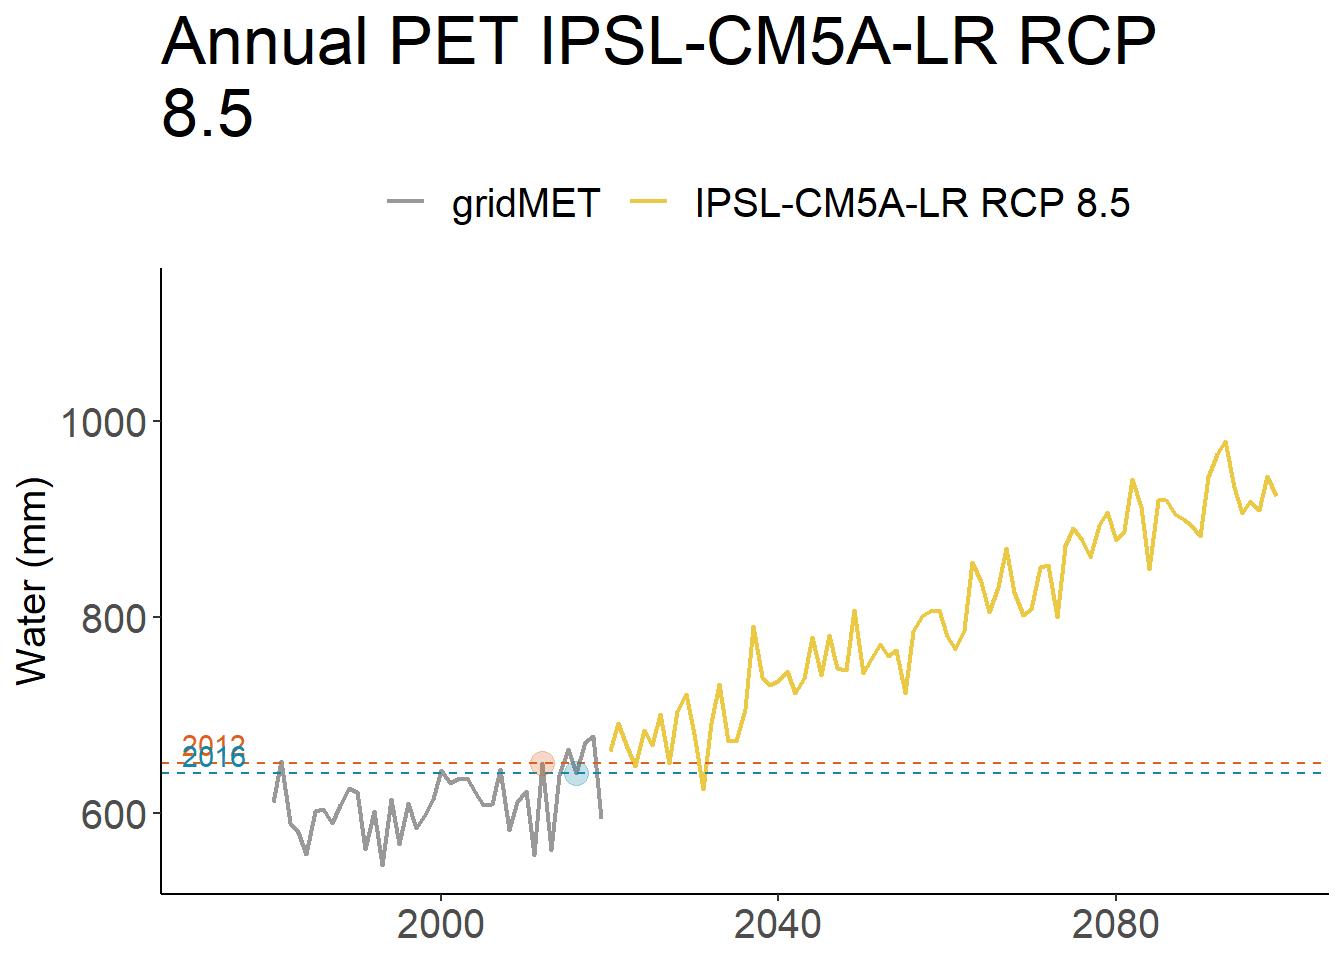
\includegraphics[width=0.5\linewidth]{water_balance_graphs_files/figure-latex/unnamed-chunk-24-4}
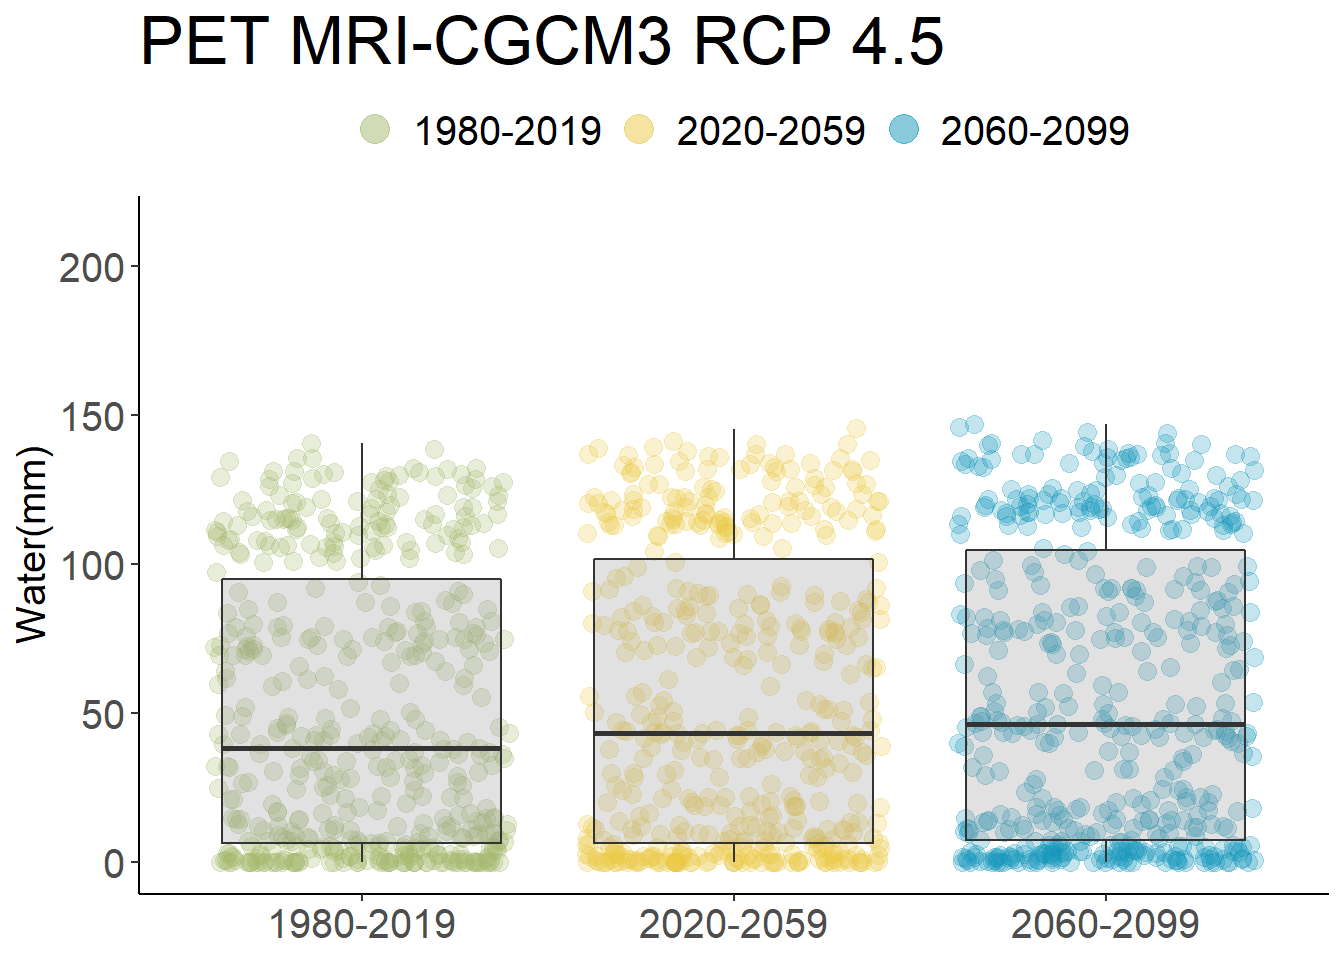
\includegraphics[width=0.5\linewidth]{water_balance_graphs_files/figure-latex/unnamed-chunk-24-5}
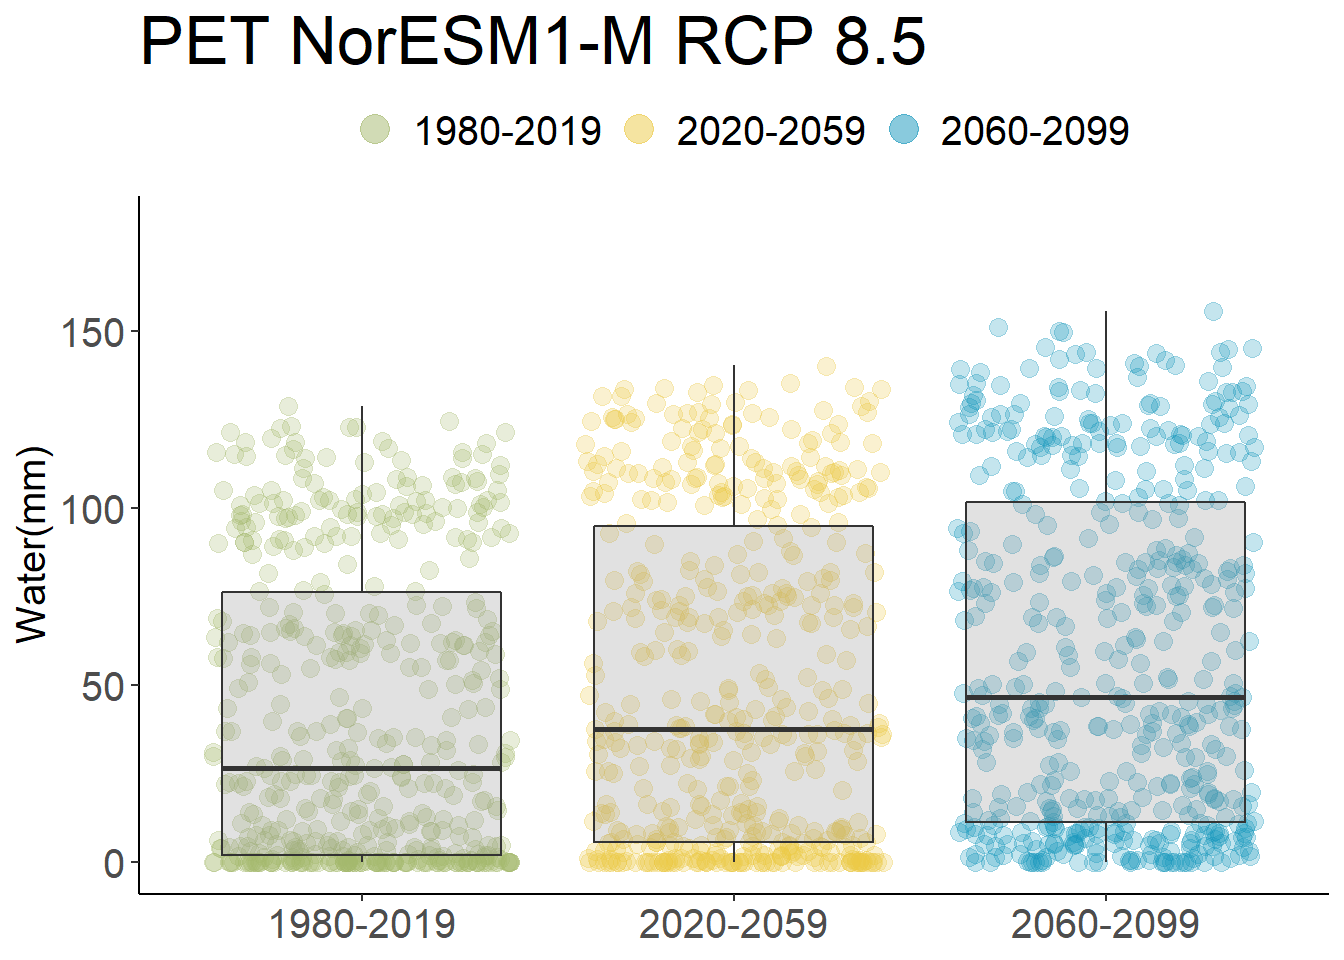
\includegraphics[width=0.5\linewidth]{water_balance_graphs_files/figure-latex/unnamed-chunk-24-6}

\hypertarget{deficit}{%
\subsection{Deficit}\label{deficit}}

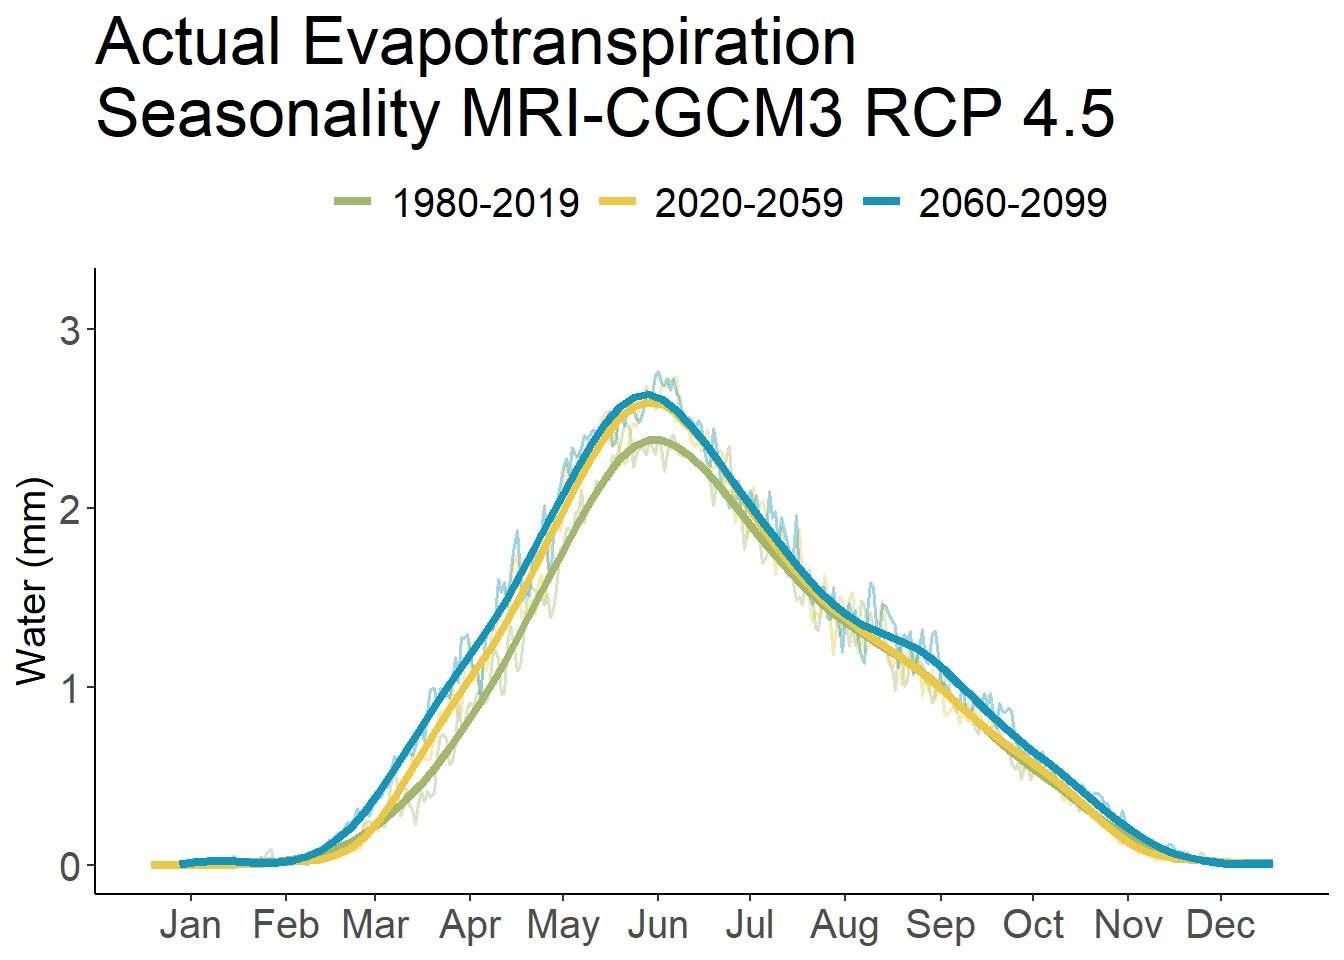
\includegraphics[width=0.5\linewidth]{water_balance_graphs_files/figure-latex/unnamed-chunk-25-1}
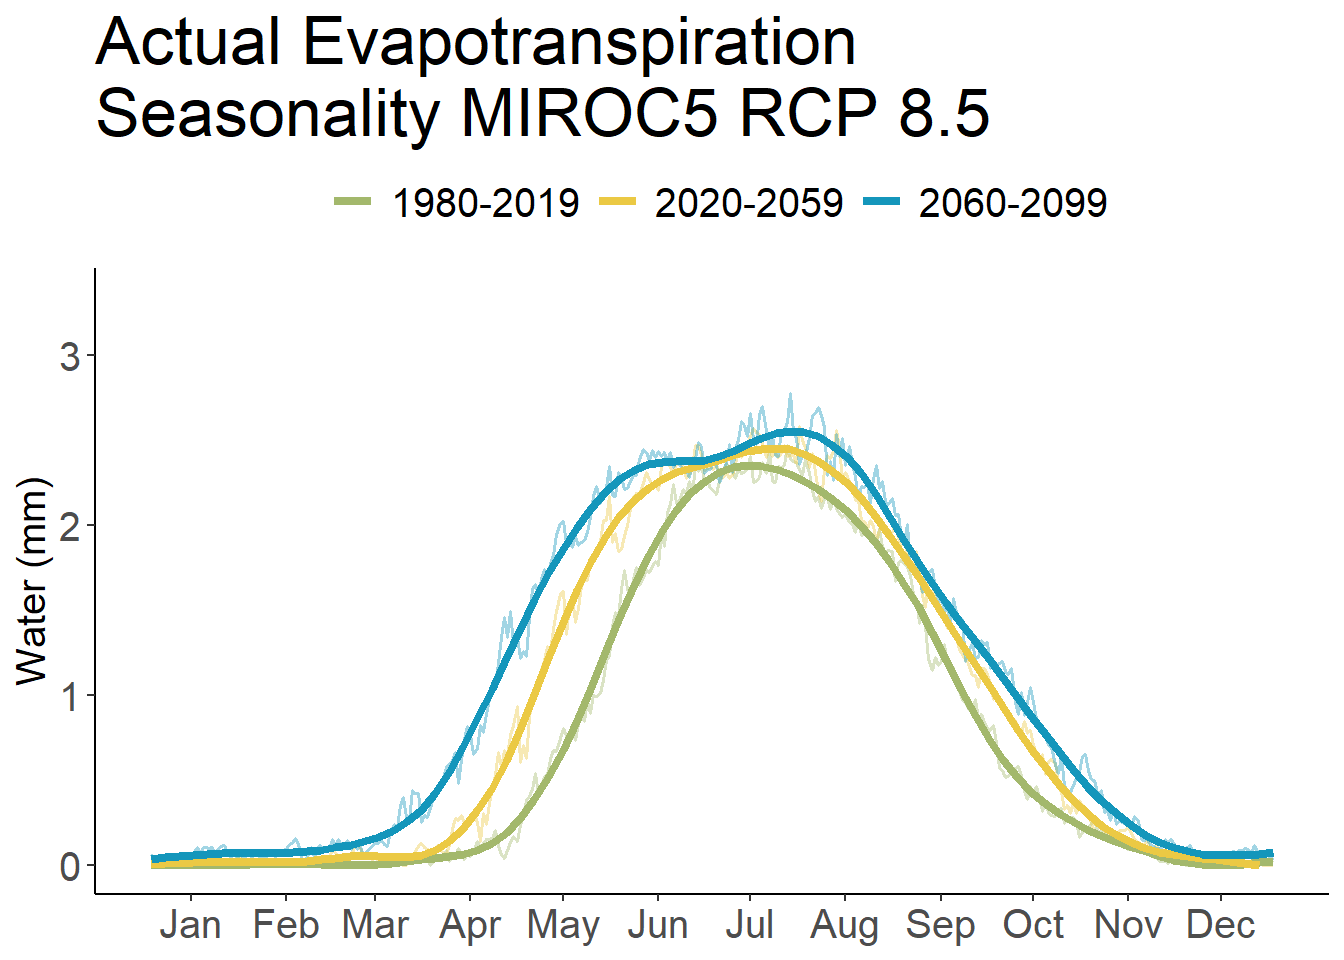
\includegraphics[width=0.5\linewidth]{water_balance_graphs_files/figure-latex/unnamed-chunk-25-2}
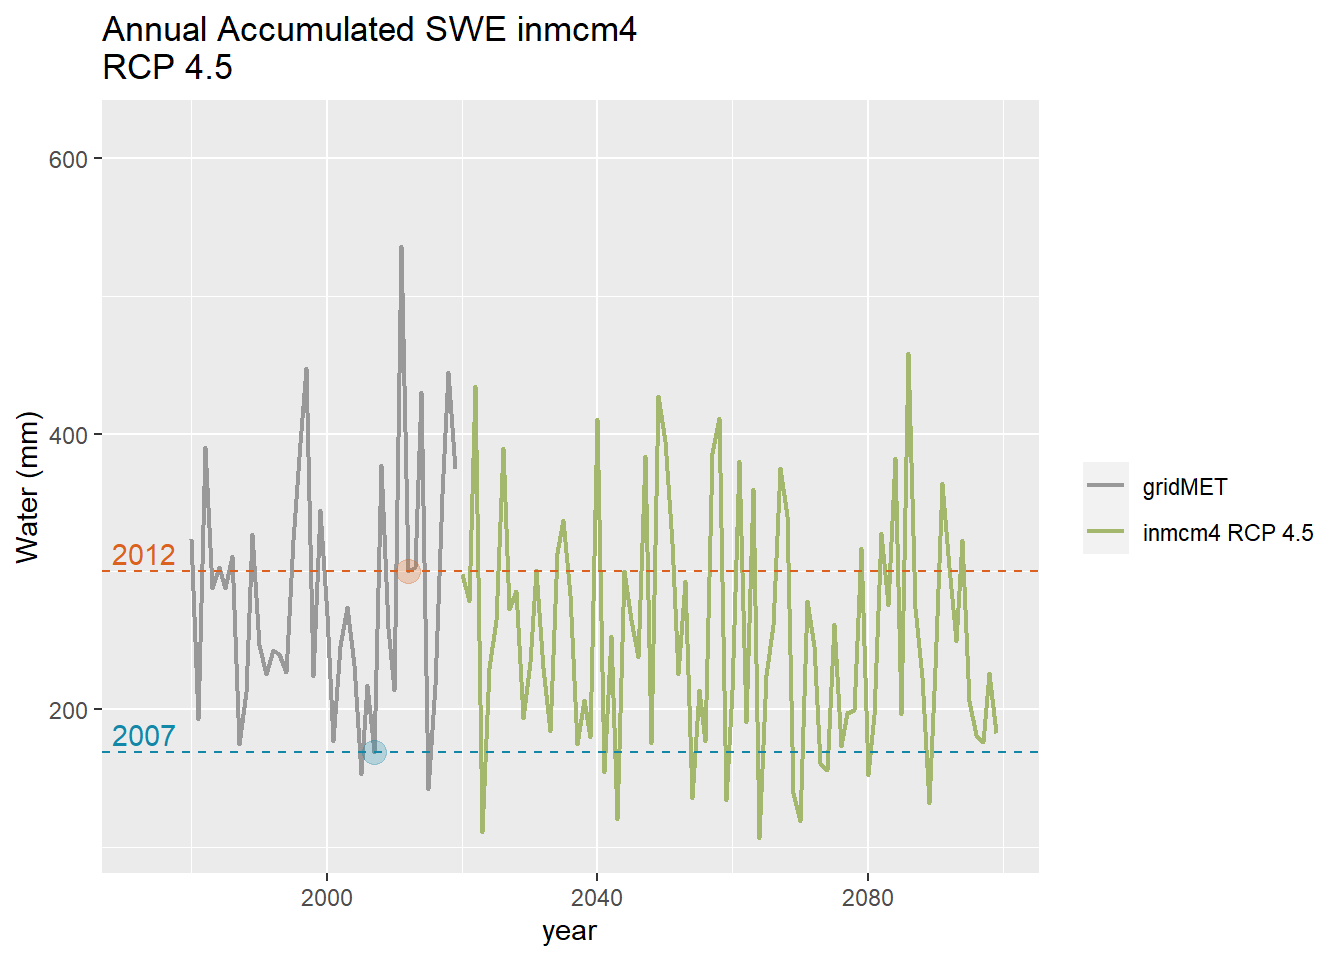
\includegraphics[width=0.5\linewidth]{water_balance_graphs_files/figure-latex/unnamed-chunk-25-3}
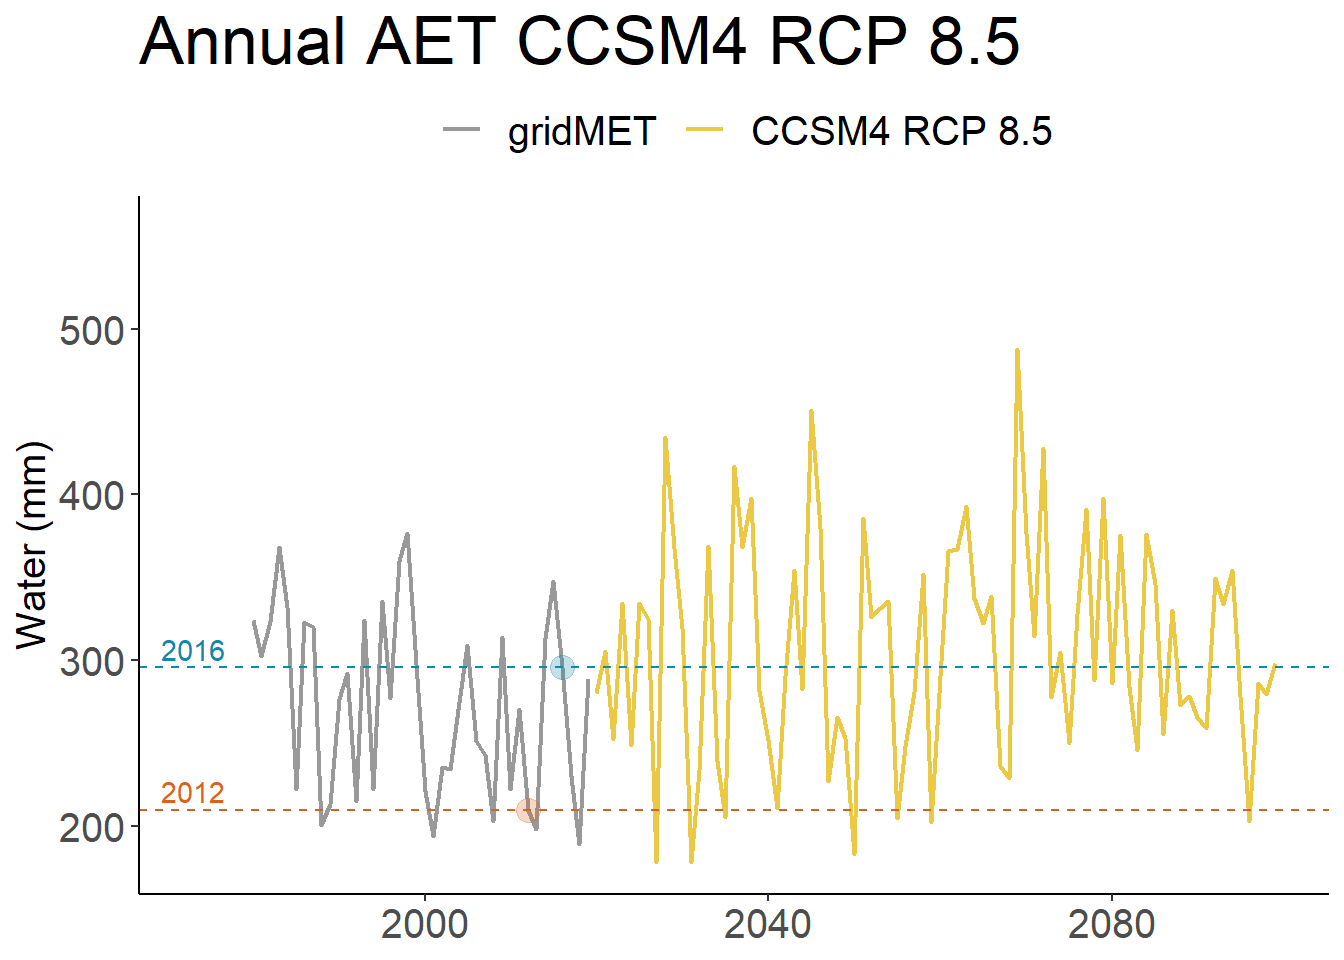
\includegraphics[width=0.5\linewidth]{water_balance_graphs_files/figure-latex/unnamed-chunk-25-4}
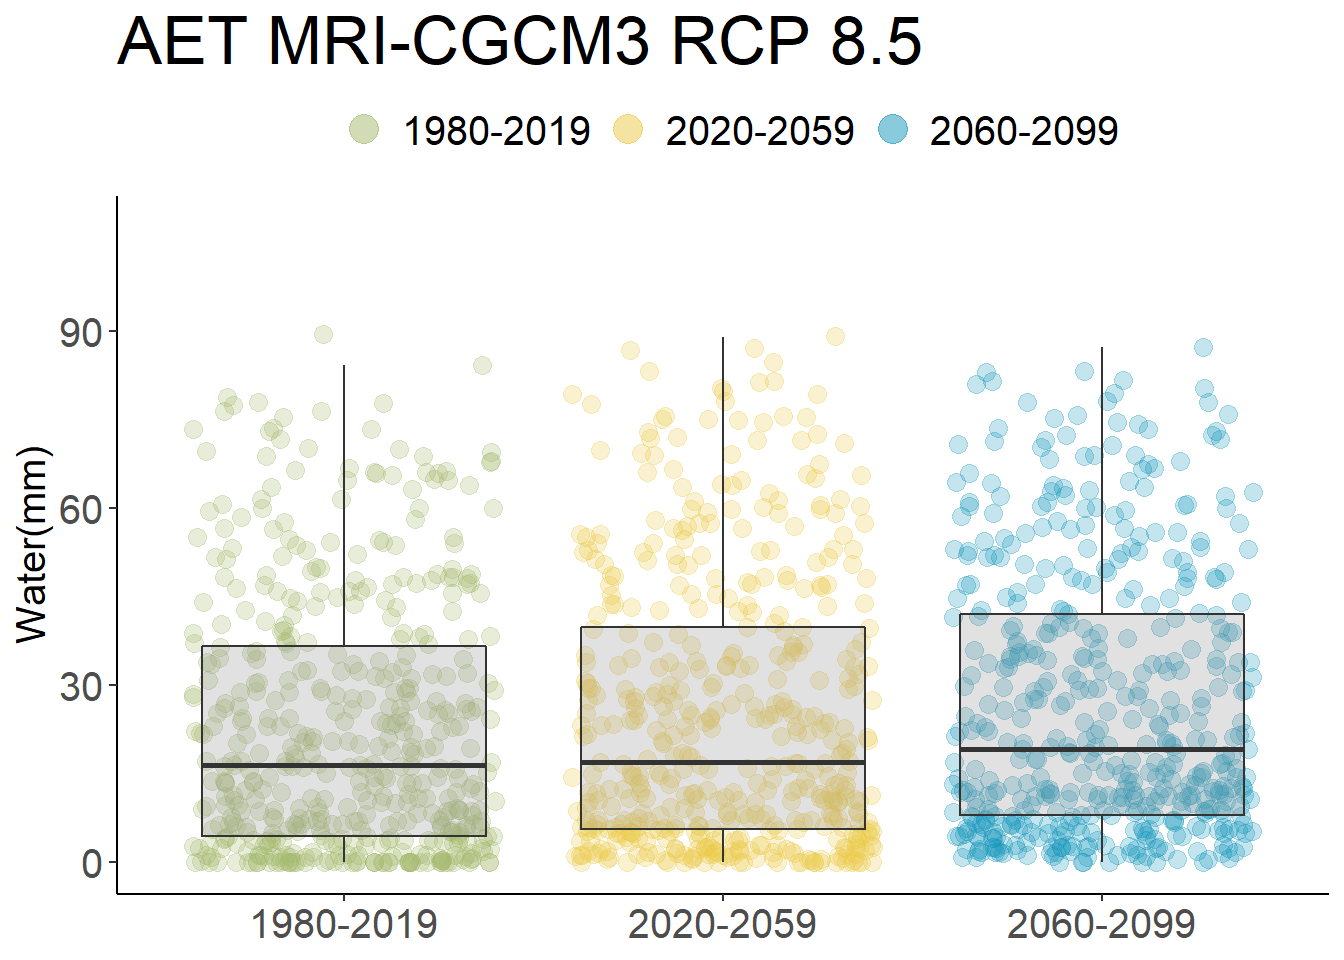
\includegraphics[width=0.5\linewidth]{water_balance_graphs_files/figure-latex/unnamed-chunk-25-5}
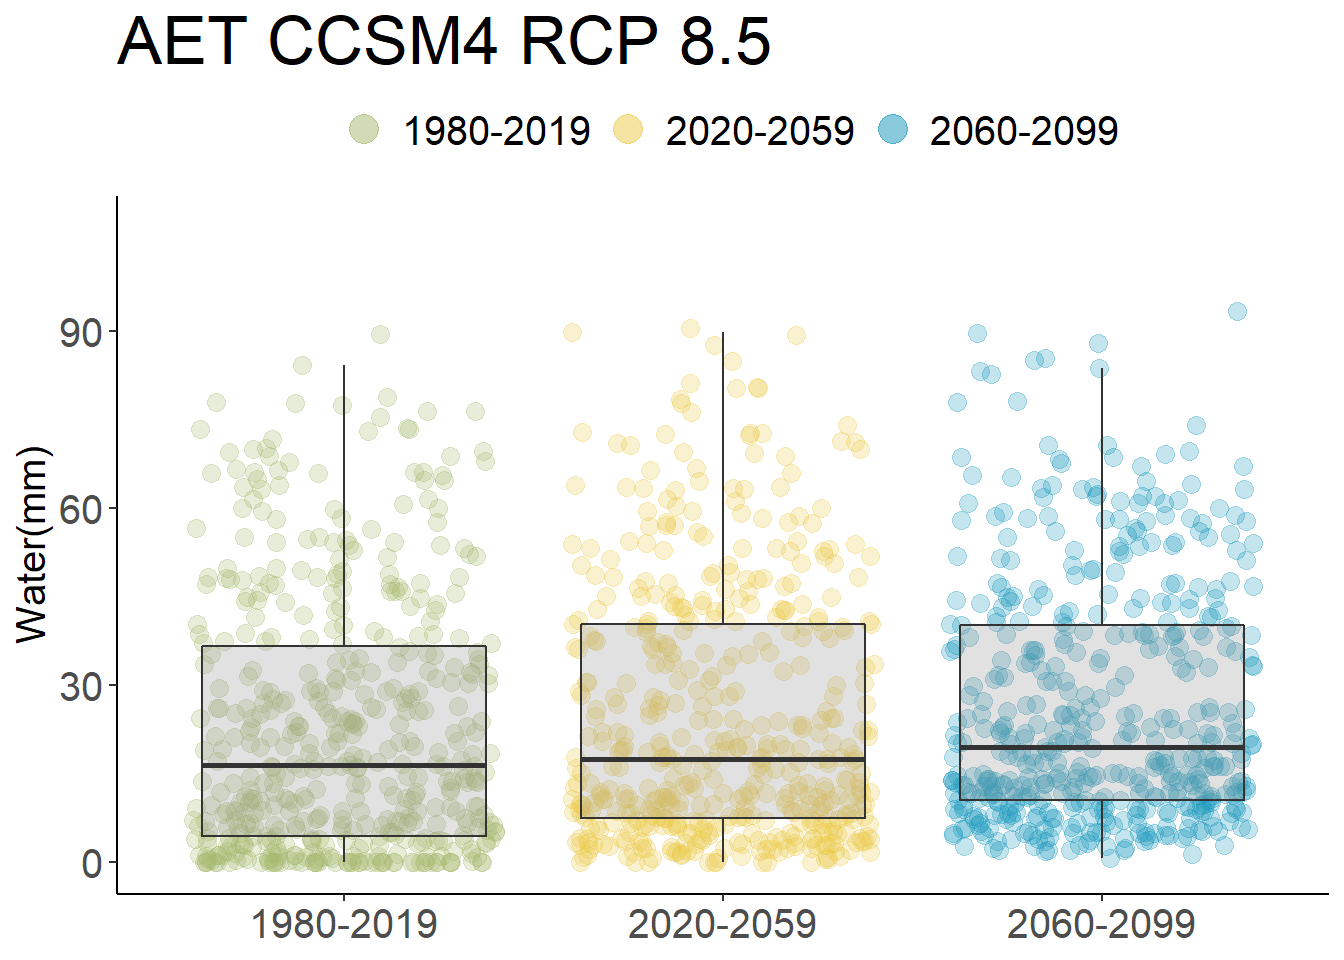
\includegraphics[width=0.5\linewidth]{water_balance_graphs_files/figure-latex/unnamed-chunk-25-6}

\hypertarget{accumulated-growing-degree-days}{%
\subsection{Accumulated Growing Degree
Days}\label{accumulated-growing-degree-days}}

\hypertarget{works-cited}{%
\subsection{Works Cited}\label{works-cited}}

Stephenson, N. (1998). Actual evapotranspiration and deficit:
biologically meaningful correlates of vegetation distribution across
spatial scales. Journal of biogeography, 25(5), 855-870.

\end{document}
